%%% File encoding: UTF-8
%%% äöüÄÖÜß  <-- keine deutschen Umlaute hier? UTF-faehigen Editor verwenden!

\documentclass[master,english]{hgbthesis}
% Zulässige Class Options:
%   Typ der Arbeit: diplom, master (default), bachelor, praktikum
%   Hauptsprache: german (default), english
%%%----------------------------------------------------------

\RequirePackage[utf8]{inputenc}		% Bei der Verw. von lualatex oder xelatex entfernen!

\graphicspath{{images/}}    % Abbildungsverzeichnis
\logofile{logo}				% Name des Logo-PDFs in images/ (\logofile{}, wenn kein Logo gewünscht)
\bibliography{literatur}  	% Name der Biblatex-Literaturdatei (.bib)

%%%----------------------------------------------------------
% Angaben für die Titelei (Titelseite, Erklärung etc.)
%%%----------------------------------------------------------

%%% Einträge für ALLE Arbeiten: -----------------------------
\title{A Selective Rendering Concept for Static Site Generators}
\author{Sascha Zarhuber}
\studiengang{Interactive Media}
\studienort{Hagenberg}
\abgabedatum{2017}{06}{26}	% {YYYY}{MM}{DD}

%%% Zusätzlich für eine Bachelorarbeit: ---------------------
\nummer{1510629021-A}   % Stud-ID, z.B. 1310238045-A
% (A = 1. Bachelorarbeit)
\semester{Sommersemester 2016}
\gegenstand{Einführung in die Tiefere Problematik 1}
\betreuer{FH-Prof. DI Rimbert Rudisch-Sommer} % oder \betreuerin{..}

%%% Restriktive Lizenformel anstatt CC (nur für Typ master) -
% \strictlicense

%%%----------------------------------------------------------
\begin{document}
%%%----------------------------------------------------------

%%%----------------------------------------------------------
\frontmatter                    % Titelei (röm. Seitenzahlen)
%%%----------------------------------------------------------

\maketitle
\tableofcontents

% \chapter{Vorwort} 	% engl. Preface


Dies ist \textbf{Version \hgbthesisDate} der \latex-Dokumentenvorlage für 
verschiedene Abschlussarbeiten an der Fakultät für Informatik, Kommunikation
und Medien der FH Oberösterreich in Hagenberg, die mittlerweile auch 
an anderen Hochschulen im In- und Ausland gerne verwendet wird.

Das Dokument entstand ursprünglich auf Anfragen von Studierenden,
nachdem im Studienjahr 2000/01 erstmals ein offizieller
\latex-Grundkurs im Studiengang Medientechnik und -design an der
FH Hagenberg angeboten wurde. Eigentlich war die Idee, die bereits
bestehende \emph{Word}-Vorlage für Diplomarbeiten "`einfach"' in
\latex\ zu übersetzen und dazu eventuell einige spezielle
Ergänzungen einzubauen. Das erwies sich rasch als wenig
zielführend, da \latex, \va was den Umgang mit Literatur und
Grafiken anbelangt, doch eine wesentlich andere Arbeitsweise
verlangt. Das Ergebnis ist -- von Grund auf neu geschrieben und
wesentlich umfangreicher als das vorherige Dokument --
letztendlich eine Anleitung für das Schreiben mit \latex, ergänzt
mit einigen speziellen (mittlerweile entfernten) Hinweisen für \emph{Word}-Benutzer.
Technische Details zur aktuellen Version finden sich in Anhang \ref{ch:TechnischeInfos}.

Während dieses Dokument anfangs ausschließlich für die Erstellung
von Diplomarbeiten gedacht war, sind nunmehr auch  
\emph{Masterarbeiten}, \emph{Bachelor\-arbeiten} und \emph{Praktikumsberichte} 
abgedeckt, wobei die Unterschiede bewusst gering gehalten wurden.

Bei der Zusammenstellung dieser Vorlage wurde versucht, mit der
Basisfunktionalität von \latex das Auslangen zu finden und -- soweit möglich --
auf zusätzliche Pakete zu verzichten. Das ist nur zum Teil gelungen;
tat\-säch\-lich ist eine Reihe von ergänzenden "`Paketen"' notwendig, wobei jedoch
nur auf gängige Erweiterungen zurückgegriffen wurde.
Selbstverständlich gibt es darüber hinaus eine Vielzahl weiterer Pakete,
die für weitere Verbesserungen und Finessen nützlich sein können. Damit kann
sich aber jeder selbst beschäftigen, sobald das notwendige Selbstvertrauen und
genügend Zeit zum Experimentieren vorhanden sind.
Eine Vielzahl von Details und Tricks sind zwar in diesem Dokument nicht explizit
angeführt, können aber im zugehörigen Quelltext jederzeit ausgeforscht
werden.

Zahlreiche KollegInnen haben durch sorgfältiges Korrekturlesen und
konstruktive Verbesserungsvorschläge wertvolle Unterstützung
geliefert. Speziell bedanken möchte ich mich bei Heinz Dobler für
die konsequente Verbesserung meines "`Computer Slangs"', bei
Elisabeth Mitterbauer für das bewährte orthographische Auge und
bei Wolfgang Hochleitner für die Tests unter Mac~OS.

Die Verwendung dieser Vorlage ist jedermann freigestellt und an
keinerlei Erwähnung gebunden. Allerdings -- wer sie als Grundlage
seiner eigenen Arbeit verwenden möchte, sollte nicht einfach
("`ung'schaut"') darauf los werken, sondern zumindest die
wichtigsten Teile des Dokuments \emph{lesen} und nach Möglichkeit
auch beherzigen. Die Erfahrung zeigt, dass dies die Qualität der
Ergebnisse deutlich zu steigern vermag.

Der Quelltext zu diesem Dokument sowie das zugehörige
\latex-Paket sind in der jeweils aktuellen Version online
verfügbar unter
%
\begin{itemize}
\item[]\url{https://sourceforge.net/projects/hgbthesis/}.
\end{itemize}
%
Trotz großer Mühe enthält dieses Dokument zweifellos Fehler und Unzulänglichkeiten
-- Kommentare, Verbesserungsvorschläge und passende Ergänzungen
sind daher stets willkommen, am einfachsten per E-Mail direkt an mich:
\begin{itemize}
\item[]%

Dr.\ Wilhelm Burger, Department für Digitale Medien,\newline
Fachhochschule Oberösterreich, Campus Hagenberg (Österreich)\newline
\nolinkurl{wilhelm.burger@fh-hagenberg.at}
\end{itemize}

\noindent
Übrigens, hier im Vorwort (das bei Diplom- und Masterarbeiten üblich, bei Bachelorarbeiten 
aber entbehrlich ist) kann kurz auf die Entstehung des Dokuments eingegangen werden.
Hier ist auch der Platz für allfällige Danksagungen (\zB an den Betreuer, 
den Begutachter, die Familie, den Hund, \ldots), Widmungen und philosophische 
Anmerkungen. Das sollte allerdings auch nicht übertrieben werden und sich auf 
einen Umfang von maximal zwei Seiten beschränken.




 % Optional. Ggf. weglassen
\chapter{Abstract}

Whereas modern content management systems provide a solid environment for dynamic content creating and editing, their dependency on external services like database services or authentication providers often complicate their abilities to scale. Additional duties for keeping them responsive in larger ecosystems are therefore often responsible for slowing down the overall workflow of a developer.

Static site generators on the other hand offer an easy solution for steadily growing websites. Their only task is to create a full-featured file structure, which contains browser-readable HTML files that do not require any on-the-fly rendering upon request. However, static site generators contain a significant drawback, as the rendering mechanism normally cannot distinguish between already present files and new content. In fact, the build time increases every time a new file is added to the source directory.

This Master's thesis therefore tries to compensate the full extent of a complete rebuild every single build cycle by providing a caching mechanism based on a selective approach, together with a remotely working REST API as wrapping interface for user-friendly interaction and improved division of work.

\chapter{Kurzfassung}

\begin{german}
Während moderne Content Management Systeme ein gut entwickeltes Umfeld für Online-Inhaltsverwaltung und -erstellung bereitstellen, sind sie doch auf eine Anzahl externer Services angewiesen. Dazu zählen vordergründig Datenbanksysteme, aber auch verschiedene Login-Mechanismen, um Zugang zu einem gesperrten Editierbereich freizugeben. Durch die Abhängigkeit von derartigen Services entsteht bei zunehmender Größe des jeweiligen Projekts ein Anstieg des Aufwands für die Verwaltung dieser Erweiterungen.

Static Site Generatoren andererseits benötigen keine externen Erweiterungen, da ihre einzige Aufgabe darin besteht, die Website-Quellcodes in eine für Webbrowser lesbare Version zu konvertieren. Allerdings haben diese Static Site Generatoren einen erheblichen Nachteil; da sie nicht zwischen bereits vorhandenen und neuen Inhalten unterscheiden können, ist jedesmal ein vollständiger Neubau der Website-Quellen notwendig.

Diese Masterarbeit soll daher einen Lösungsweg für dieses Problem aufzeigen. Durch einen selektiven Algorithmus sollen am Ende nur die wirklich notwendigen Inhalte gebaut werden und in eine vorhandene Dateistruktur eingebunden werden. Zusammen mit einer REST API soll zusätzlich eine benutzerfreundliche Interaktion und verbesserte Arbeitsteilung möglich sein.
\end{german}


%%%----------------------------------------------------------
\mainmatter          % Hauptteil (ab hier arab. Seitenzahlen)
%%%----------------------------------------------------------

% Here comes the introduction
\chapter{Introduction}
\label{cha:introduction}
Back in the early 1990s, when the internet made its first steps towards a broader public use, a group of students at the University of Illinois created ``Mosaic'', the first publicly available Browser \cite[11]{dhillon2016}. At that time, websites consisted of just HTML and probably some images, whereas the release of ``Netscape Navigator'' led to the introduction of \emph{Brendan Eich}'s JavaScript engine. Additionally, Netscape also introduced a web server software called ``Netscape Enterprise Server'', thus making the Internet available for the first web developers \cite[12]{dhillon2016}.

Since then, a lot has changed; content management systems were published, the internet was turning to what was called ``Web 2.0'' and the common user was not just a content recipient anymore, but also a content creator without requiring deeper understanding of web technologies \cite[19]{dhillon2016}. This has affected not only private users, but also whole enterprise structures until today.

However, the most important part stayed the same; steadily providing content which is deliverable on request. To do so using content management systems requires not only a web server and the client's browser, but also a properly set up chain of interacting services for assembling HTML code on the fly. While this kind of architecture may surely be fitting smaller blogs very well, the necessary effort of managing constantly growing enterprise sites is likely to grow exponentially.

Therefore, systems which are not dependent on such a chain are constantly on the rise over the last yars. They especially make sense in environments, where content is constantly added, but hardly ever deleted or changed. Lastly, by constructing static websites in plain HTML and mostly avoiding any dynamic features, a trend reversal back to the internet origins is clearly noticeable in some fields of modern web development.

\section{Problem statement}
\label{sec:staticsitegenerators}
Static site generators are growing fast and are more and more used as a replacement for common content management systems. The main advantage is their independence of external services, like database systems, session caching services, etc. Also, they seldomly consist of complicated backend systems and are mostly created in pure HTML or simple markup languages like Markdown (see Sec. \ref{sec:buildpipelines-markdown}).

One of the biggest drawbacks however is the fact, that static site generators have to preprocess every bit of information they contain. This is the complete opposite compared to other content management systems, which process information on request. This means, that user-readable content is fetched and rendered ``just in time'' it was requested from the client.

Therefore, depending on the setup, a dynamically growing amount of time needed for a build cycle might be the case. For being able to work against this fact, a working approach has to be found, which saves time by leaving out information, which has not changed since the previous build.

\section{Goals}
\label{sec:goals}
To find a suitable solution, a service which contains a build pipeline including a caching mechanism has to be implemented. The caching mechanism should thereby act as the core part, as it is responsible for fetching data between the current development state and a previous build cycle. Furthermore it should determine the build extent by selecting the respective files for rendering based on the fetched commit diff. The research question is therefore the following:

\begin{center}
  How to speed up static site generation by a selective approach?
\end{center}
The implemented solution covers the necessary steps for working with cacheable content in a way, that a remote-only building process is possible. Together with the precondition of having a GitHub account, any repository consisting of a Metalsmith project should be able to get rendered on this service's REST API.

By introducing this service early into a project workflow, the user should notice a significant improvement concerning the rendering time per build cycle. Furthermore, it should take a considerable amount of workload out the developers hands.

\section{Structure}
\label{sec:structure}
To express the considerations which led to the finished solution, the following pages are structured into several chapters.

\begin{description}
  \item[Chapter 2] -- Shows the current state of the art, culminating in the presentation of three selected static site generators: \emph{Jekyll}, \emph{Hexo}, \emph{Metalsmith}, as well as a comparison between them.
  \item[Chapter 3] -- Explains the most important terms concerning the operation of static site generators (including code samples); \emph{build pipelines}, \emph{frontmatter}, \emph{markdown}, \emph{templates} and \emph{diff}.
  \item[Chapter 4] -- Gives an understanding of the initial theoretical approach behind this project. Challenges and solution strategies are examined prior to general considerations towards the implementation are being unveiled.
  \item[Chapter 5] -- Describes the full extent of the implementation including the whole REST framework, which was built around the build pipeline. Different graphics are showing examples of how various parts were realized.
  \item[Chapter 6] -- Evaluates the project using different testing approaches. The REST API was put under high load testing, whereas the build pipeline and the caching mechanism were compared using the timespan needed for an operation. Furthermore, an outlook shows possible future improvements.
  \item[Chapter 7] -- Shows the conclusion of this project work and unveils difficulties, as well as enhancement strategies for productive use.
\end{description}

% Transforming Web 1.0 to Web 2.0 - common user is not only content recipient anymore, also content creator
%% in the beginning, creating content on the internet was too difficult for the average Joe.

% Web 2.0 standards-based web, one way to measure is content creation
%% Blogs, social media, videos

% Blogging emerged as a solution to one of the biggest problems; not having enough people to create content

% Not just blogging software, also computer languages evolved

% Blogging will never die out, simply will take over a new form

\chapter{State of the art}
\label{cha:state-of-the-art}

%% W3Tech chart of server-side language share
\begin{figure}
    \centering
    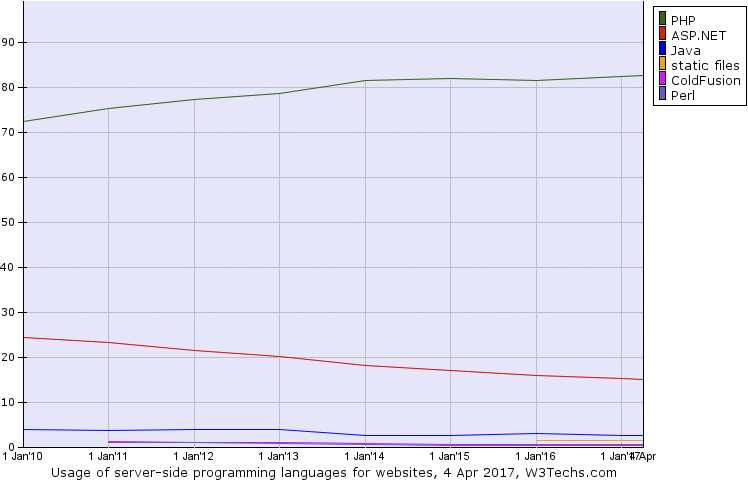
\includegraphics[width=0.9\textwidth]{server-side-languages.png}
    \caption{A graphic showing the global share of \emph{server-side programming languages} from January 2010 to April 2017. \emph{PHP} remains the dominant language with a share growing from 72.5\% to 82.6\%.\\
    Source: \url{https://w3techs.com/technologies/history_overview/programming_language/ms/y}}
    \label{fig:server-side-languages}
\end{figure}
%

\paragraph{} % History of Content Management Systems.
The roots of the most well-known modern Content Management Systems (\emph{CMS}) date back to the early 2000s, when PHP was (and \emph{still is}) the dominant factor in terms of server-side programming languages (see Fig. \ref{fig:server-side-languages}). %% Please check, if reference is accurate enough

While the \emph{typical} CMS was starting out as mostly just a ``dynamic online tool'', it also shows that with seamlessly integrating new features gained through the development of its underlying programming languages, as well as steadily adding new functionalities (mostly requested by the community), a transition towards a fully-manageable and customizeable, semi-automatic web application was possible \cite[17]{dhillon2016}.

The advantages are clear; A web designer or content editor does not automatically have to be a web developer, who needs profound knowledge about software or server architecture. Instead, most of the time it is enough to know how to operate an FTP-client and to know the credentials of the built-in database service, submitted by the web hosting provider upon registration.\\
As a summary, it can be said: \emph{Less people for less responsibilities} -- The web application does the rest.

However, this progression also caused a few drawbacks, especially when it comes down to comparing the amount of workload needed before actually being able to create content for the World Wide Web. Due to the fact, that most CMSs evolved to their own sort of powerful admin panels, developers who are not keen about keeping their site updated, risk its defacing or other embarrassing attacks through unmanaged security holes in the code \cite[23]{dhillon2016}.\\
So, how is it possible to bridge the gap between a fairly secure system and creating content whenever it is desired?

\paragraph{} % Creating content using static HTML.
\label{par:creatingcontent}
In 2008, \emph{Tom Preston-Werner} created \emph{Jekyll} out of his frustration of having the need of ``styling a zillion template pages'' and ``moderating comments all day long'' before even being ready to create content on his blogging engine \cite[]{PrestonWerner2008jekyll}. Furthermore he mentioned, that one of the other main reasons were the lack of possibility for publishing his posts on his own server, when subscribing to a fully-managed online hosting service like \texttt{wordpress.com}\footnote{\url{https://en.wordpress.com} -- A hosted version of Wordpress.}. Services like this offer only limited customization options, where there likely is no access to online storage and database without using the built-in admin panel. Even then, access might be very restricted.

The intended core functionality of Jekyll narrows down its mode of operation to handle three main components found in most static site generators today \cite[24]{dhillon2016}:

\begin{description}
  \item [Core language] -- The language a static generator is written in, for example JavaScript or Ruby.
  \item [Templates] -- The templating language to be used through the blog and posts.
  \item [Plug-ins] -- All static site generators allow for additional functionality through some
sort of a plug-in system.
\end{description}

In contrast to common dynamic CMSs, a static site generator outputs plain static HTML. It does it in a way, that a certain \emph{distribution} folder holds the complete web root, without the need of binding it to external services like databases or session management tools. Occasionally, different plug-ins also allow the generation of client-side \emph{JavaScript} or \emph{Cascading Style Sheet} files through their respective pre-processing tools.

\section{Jekyll}
\label{sec:jekyll}

As already explained, Jekyll was created out of the need for avoiding to service the blogging engine before writing and publishing content. Since it is deeply integrated into \emph{GitHub}, it is considered as the probably most-popular static site generator.

\subsection{History}
\label{sec:jekyll-history}
\emph{Tom Preston-Werner}, co-founder of GitHub\footnote{\url{https://github.com} -- GitHub Inc.}, announced it in October 2008 in one of his blog posts \cite{PrestonWerner2008jekyll}. Already in December 2008, it was introduced as build engine for the then newly featured GitHub Pages service, allowing owners of repositories to publish a static website by just pushing to a certain \emph{master} or \emph{gh-pages} branch \cite{PrestonWerner2008githubpages}, which is still available for free to this day.

All of this happened just 6 (respectively 8) months after GitHub was launched \cite{PrestonWerner2008githublaunch} and is now even being used by technology-leading companies to showcase their Open-Source efforts\footnote{\url{https://github.com/showcases/github-pages-examples} -- GitHub Pages examples.}.

\subsection{Technology}
\label{sec:jekyll-technology}
Jekyll was entirely written in \emph{Ruby}, as Tom Preston-Werner rather saw himself as a software developer in the first place, than as a content author \cite{PrestonWerner2008jekyll}. Until now, the repository for Jekyll still consists mainly of Ruby code at a share of roughly 77.5\%.

\subsubsection{Advantages}
One of the main advantages is the modular structure of its code base. By inheriting different Ruby classes, it is quite easy to extend and add features to fit the developer's needs. Due to its wide-spread usage initiated through the GitHub universe, Jekyll also has an accordingly huge user base and is therefore well documented \cite[26]{dhillon2016}.

Furthermore, its website\footnote{\url{http://jekyllrb.com} -- Jekyll website.}, which mainly acts as starting basis for documentation, is not only available as open-sourced git repository, it is also built using \texttt{Jekyll} to prove its universality.

Starting from scratch, the command \texttt{jekyll new my\_project} installs a blog environment for starters in the \texttt{./my\_project} folder. The basic install consists of an elementar blog post structure, \emph{Sass} source files, and a few template files written for Shopify's \emph{Liquid}\footnote{\url{https://help.shopify.com/themes/liquid} -- Shopify's Liquid template engine.} engine.\\
Using this starting environment, the unexperienced developer quickly gets a sufficient overview of what is generally possible using Jekyll, whereas the content author is able to fully concentrate himself on writing content, as the used \emph{Markdown} markup language requires little to no prior syntax knowledge. Furthermore, Jekyll already ships with a built-in webserver for quickly reviewing the rendered static output.

\subsubsection{Disadvantages}
As powerful as Ruby might be designed, many unskilled developers are facing difficulties right from the beginning, as most of them experience a steep learning curve. Nearly every single bit of customizing Jekyll requires Ruby knowledge, especially if it is desired to move along the ``predefined'' way and not including third-party extensions like \emph{Node.js} tools or else.

Additionally, its template language, Liquid, offers customization on a very high level, so it might happen to confuse business logic\footnote{How Jekyll processes data into programmatically readable structures.} with template logic\footnote{How Liquid transforms these structures into browser-readable HTML.}. To make things worse, different template constructions might also evolve over time and therefore causing a parallel coding universe when trying to surpass difficulties in the business logic.

%% bring some difficulties concerning ruby versions
%% ruby gems

\section{Hexo}
\label{sec:hexo}

\texttt{Hexo} understands itself as counterpart to \texttt{Jekyll}, mostly by covering the same ideas of static site generation, but building up completely on \texttt{Node.js}. It even offers a migration service for \texttt{Octopress}- and \texttt{Jekyll}-users who are willing to switch.

\subsection{History}
\label{sec:hexo-history}
\texttt{v1.0.0} was originally released in March 2013\footnote{\url{https://github.com/hexojs/hexo/releases/tag/1.0.0} -- Hexo v1.0.0 release page on \texttt{GitHub}.}, although development on \texttt{GitHub} dates back to September 2012 as the first commit was published using the message \emph{``init''}.

\emph{Tommy Chen}, its creator, first used \texttt{Octopress}\footnote{\url{http://octopress.org} -- Octopress website.} but quickly became dissatisfied with its performance, as the rendering of 54 blog posts already took more than a minute of compile time \cite{Chen2012hexodebut}. Since he assumed \texttt{Ruby} might be the cause for the lack of performance of his primarily used blogging framework, and further development on this case was not likely to happen any time soon, he decided to look for something which got his attention shortly before: \texttt{Node.js}.

However, \texttt{Node.js} was not really a big player back at that time, so the offer of blogging frameworks written in \texttt{JavaScript} was very dense and not really fitting the needs of \emph{Tommy Chen}. In his announcement article for \texttt{Hexo} \cite{Chen2012hexodebut}, he references a blog post of \emph{Boris Mann}, also an \texttt{Octopress} user at that time, listing a few \texttt{Node.js}-based blogging frameworks, which were already around in June 2012\footnote{\url{http://blog.bmannconsulting.com/node-static-site-generators} -- Blog article of \emph{Boris Mann} about \texttt{Node.js}-based blogging frameworks.}. Interestingly, only two of all the mentioned ones, \texttt{Wintersmith} and \texttt{DocPad} are still actively maintained today.

\subsection{Technology}
\label{sec:hexo-technology}
As already stated above, \texttt{Hexo} primarily consists of \texttt{JavaScript}, thus making it easier to start for developers with a front-end web development background. In fact, its \texttt{GitHub} repository shows \texttt{JavaScript} holding a share of 100\% on the source code\footnote{\url{https://github.com/hexojs/hexo} -- Hexo repository on \texttt{GitHub}.}.

\subsubsection{Advantages}
Right from the start, \texttt{Hexo} presents itself using its feature-rich command-line interface (\emph{CLI}), similar to \texttt{Jekyll}. Once it is installed, \texttt{hexo init my\_project} scaffolds a new starter template into the \texttt{./my\_project} folder.\\
As \emph{Tommy Chen} himself wanted an easy-to-use replacement for \texttt{Octopress}, \texttt{Jekyll} and \texttt{Hexo} share a lot of common features; their content files use both \texttt{YAML} frontmatter and \texttt{Markdown} by default, even the main configuration file uses a very similar structure in both frameworks. This should make it extremely easy switching from \texttt{Jekyll} to \texttt{Hexo}.

First and foremost, programming-unaware content authors might especially like its CLI, as it also offers to create files based on the \texttt{hexo new} command. Depending on other submitted command-line arguments, \texttt{Hexo} may automatically put the new post in the according sub-folder, whether it is a \emph{draft, page} or \emph{post}. Publishing a draft is as easy as \texttt{hexo publish}.\\
When creating content, \texttt{Hexo} also contains a feature-rich, \texttt{Octopress}-inspired custom tag selection for including content from \emph{YouTube, Vimeo} or \emph{GitHub Gists}.

Additionally, its plugin collection is also constantly growing and mostly community supported. A special naming convention using \texttt{hexo-} as prefix helps by determining which plugins to auto-load out of the \texttt{node\_modules} folder. Using this way, \texttt{Ruby's} \emph{convention over configuration} mantra is ported to \texttt{JavaScript} as well and supports especially beginners by not having to define the usage of a certain plugin.

\subsubsection{Disadvantages}
\texttt{Hexo} might look like as an ideal replacement for \texttt{Jekyll}, but since both share so much similarities, they also share some disadvantages. Whereas \texttt{Jekyll} ships with \emph{Liquid} and \emph{Sass} as standard, \texttt{Hexo} does with \emph{EJS} and \emph{Stylus}.\\
Although clearly stated, that both of these plugins might be easily uninstalled later on\footnote{\url{https://hexo.io/docs/setup.html\#package-json} -- Hexo's setup documentation.}, the whole setup pre-installation seems as opinionated as \texttt{Jekyll's}.

In addition to the already mentioned plugin system, a missing configuration option might as well turn out to be misleading in terms of customization options, especially when being dependent on the CLI. If customization is necessary, the developer often is forced to switch to the \texttt{JavaScript} API\footnote{\url{https://hexo.io/api/} -- Hexo's JavaScript API documentation.} or add a plugin to the project to make the build pipeline fit the customization's needs.

When it comes to caching, \texttt{Hexo} uses a homebrew version of \emph{JSON memory caching} called \texttt{Warehouse}, also created by \emph{Tommy Chen}\footnote{\url{https://github.com/tommy351/warehouse} -- Warehouse repository on \texttt{GitHub}.}, initially mentioned in the release notes of \texttt{3.2.0-beta.2} \cite{Chen2015hexorelease}. Using this plugin, a mode called ``Hot processing'' should enable faster re-builds. The main drawback here might be the caching speed, which is on the one hand filling up the memory when working on bigger projects, whereas the persisting of the database is fully dependent on file input/output write speeds of the underlying hard disk.\\
Furthermore, a constantly growing database file is hardly transferrable when trying to implement a decentralized building system out of \texttt{Hexo}.

\section{Metalsmith}
\label{sec:metalsmith}

Compared to the already described static site generators, \texttt{Metalsmith} is to be considered the youngest project.
It might also be the most radical project, as it was designed to consist of \textbf{nothing but plugins} \cite[31]{dhillon2016}. Therefore, in terms of still being a static site generator, it tries hard to push the limits much further than previously mentioned \texttt{Jekyll} and \texttt{Hexo}.

\subsection{History}
\label{sec:metalsmith-history}
Initially developed by \emph{Segment}\footnote{\url{https://segment.com} -- Segment's website.} for their internal needs, such as \emph{documentation, help} and \emph{blog pages} \cite{Metalsmith2015buildingblocks}, \texttt{Metalsmith} was finally open-sourced and made publicly available around February 2015 -- its commit history on \texttt{GitHub} dates back to February 4\textsuperscript{th}, 2014.\\
Most of the commits at that time were published by \emph{Ian Storm Taylor}, co-founder of \emph{Segment}, although his contribution to the project ends after releasing \texttt{v2.1.0} on September 24\textsuperscript{th}, 2015\footnote{\url{https://github.com/segmentio/metalsmith/commits/master?author=ianstormtaylor} -- Contributions of \emph{Ian Storm Taylor} to the Metalsmith repository on \texttt{GitHub}.} at the moment.

Like \texttt{Hexo}, \texttt{Metalsmith's} repository completely consists of \texttt{JavaScript} code, as its developers also were unsatisfied with the then existing static site generators. According to \emph{Chris Sperandio}, the \texttt{Metalsmith} developers desired pure flexibility for their ``wide array of use cases'', while other frameworks all asked for a certain structure on the content \cite{Metalsmith2015buildingblocks}.

\subsection{Technology}
\label{sec:metalsmith-technology}
Since \texttt{Metalsmith} consists of only plugins, specifically written for this very framework, there is no real standard setup provided. Although there are a few tutorials and best practices listed in its \texttt{GitHub} repository\footnote{\url{https://github.com/segmentio/metalsmith\#the-secret} -- Possibilities for using Metalsmith.}, as well as in a repository called ``\emph{awesome-metalsmith}''\footnote{\url{https://github.com/metalsmith/awesome-metalsmith} -- ``Awesome'' Metalsmith resources list.}, the initial dive-in might scare a few people away, since \texttt{Metalsmith} might not be as well documented as the previously mentioned frameworks. Moreover, most developers seem to experience a very steep learning curve at first, given the amount of customization options and the requirements for understanding the blog engine~infrastructure \cite[31]{dhillon2016}.

\subsubsection{Advantages}
Every developer is able to shape \texttt{Metalsmith} exactly to his/her needs, once he knows about the basic usage. It ships with a CLI, as well as a \texttt{JavaScript} API, where the ``real hacking'' is possible.\\
The CLI gets easily configured via a \texttt{metalsmith.json} file, stored in the project directory. It consists mainly of general project configurations, placed in the object's root, as well as an array of used plugins, respectively combined with their configuration.

It neither contains a pre-installed template engine, nor any other pre-processing tools, like \texttt{Sass} or \texttt{Less}. However, the available plugins support most of them to a satisfying extent. As an example, the \texttt{metalsmith-layouts} plugin is a wrapper for \texttt{consolidate.js}, which per se acts as a wrapper for the most common template engines\footnote{\url{https://github.com/tj/consolidate.js\#supported-template-engines} -- Consolidate.js-supported template engines on \texttt{GitHub}.}. Therefore, the developer is able to select the tools based on his/her preferences and may initialize a project from scratch, without needing to clean up any pre-installed demonstration files first.

Using the built-in \texttt{JavaScript} API, it is also possible to invoke the needed modules programmatically, which is one of the core topics of this Thesis.

\subsubsection{Disadvantages}
So much freedom in designing a project may also cause some dangers. In this case, one of the most crucial things is the arrangement of plugins in the configuration. Since \texttt{Metalsmith} acts as a streaming build system, every transformation of the content must happen at its time to not interfere with any upcoming plugins. This is especially important when a plugin might alter the underlying code in a way, that a following plugin becomes useless, as it might not be able to succeed in its predefined task. \emph{Andy Jiang} gives a good example about a sample structuring of \texttt{Metalsmith} plugins on the \emph{Segment} blog \cite{Metalsmith2015technicaldocumentation}.

As an example, the following code snippet shows one bold example of misconfiguration (See line no. 16):

%% Update line no. above, if code changes
\lstinputlisting[language=JavaScript]{chapters/02-state-of-the-art/_support/metalsmith.js}

%% Screenshot of npms.io for search query metalsmith static assets
\begin{figure}[b] % h-ere, t-op, b-ottom, p-age
    \centering
    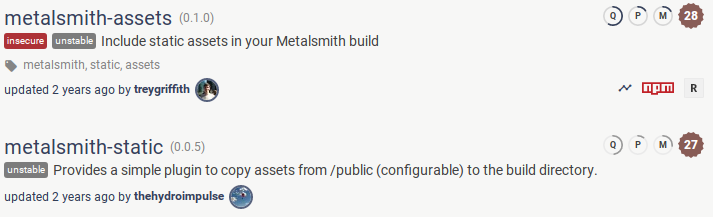
\includegraphics[width=0.9\textwidth]{metalsmith-static-plugins.png}
    \caption{A screenshot showing some of the results for the search query ``\emph{metalsmith static assets}'' on \url{https://npms.io}. Both of the shown entries describe an identical mode of operation within the \texttt{Metalsmith} build pipeline.\\
    Also notice the very unstable \texttt{semver} versions: \textbf{0.1.0} and \textbf{0.0.5}.}
    \label{fig:metalsmith-plugins}
\end{figure}
%

Moreover, the available plugins may seem as not as popular as the plugins from \texttt{Hexo}, given the average amount of stars received on \texttt{GitHub}. This might be due to the often missing maintainance, or simply because of the fact, that there seem to be multiple plugins for one single task (See Fig. \ref{fig:metalsmith-plugins}).

\section{Comparison}
\label{sec:comparison}

To conclude the summaries of different static site generators, a short overview using a table is given below (see Table \ref{table:comparison}). The comparison is built up on advantages and disadvantages, as well as the most important features they consist of. Therefore overall popularity and customizability play an as important role, as the language they are written in. However, Metalsmith stands a little bit out, as it does not provide a full-featured framework -- it merely serves as the basis for further plugin setup, whereas Jekyll and Hexo already contain some sort of standard setup.
The numbers of plugins in Table \ref{table:comparison} were taken from search queries on \url{https://npms.io} and \url{https://rubygems.org}.

\begin{table}
  \caption{A comparison of static site generators}
  \label{table:comparison}
  \centering
  \setlength{\tabcolsep}{5mm}
  \def\arraystretch{1.25}
  \begin{tabular}{|r||c|c|c|}
    \hline
    & \emph{Jekyll} & \emph{Hexo} & \emph{Metalsmith} \\
    \hline
    \hline
    Language & Ruby & JavaScript & JavaScript \\
    \hline
    Foundation & Oct. 2008 & Sept. 2012 & Feb. 2014 \\
    \hline
    Contributors & \textasciitilde 700 & \textasciitilde 100 & \textasciitilde 50 \\
    \hline
    Plugins & \textasciitilde 800 & \textasciitilde 600 & \textasciitilde 590 \\
    \hline
    Customizability & Mediocre & Low & High \\
    \hline
    Opinionatedness & High & High & Low \\
    \hline
    Standard templates & Liquid & Swig & \emph{none} \\
    \hline
  \end{tabular}

\end{table}


\chapter{Technical foundations}
\label{cha:technicalfoundations}

Before any explanation of the theoretical approach behind this research, there is a need of describing the technical foundations, on which the general thoughts were built on.

Being mostly a back-end web developer, one surely gets confronted with a lot of changes in this field. Changes which were mostly caused by the ongoing progression of general web development, but also caused by constantly coming and going ``hypes''. Changes which might leave minor traces, but sometimes also having a major impact on the way some developer processes things during his/her work on different projects.

\paragraph{} % EcmaScript 6.
One of these major turning points was the introduction of EcmaScript 6 (\emph{ES6}), which provides a more sophisticated application flow for software developers compared to the old standards, where the code architecture quickly got out of hand, especially if not fastidiuosly checked using \emph{JSLint} \cite{JSLintDocumentation}. ES6 introduced a lot of new features, pushing JavaScript more and more towards the definition of an ``object-oriented'' scripting language, thus not only by providing ``real classes'', instead of the old and cumbersome approach of inheritence by setting a constructor function into the \emph{prototype} object \cite[47]{crockford2008javascript}.

However, the probably most beneficial functions are \emph{Promises} \cite{MDNPromise} and \emph{Arrow functions} \cite{MDNArrowFunctions}, both saving significant amounts of code -- especially when working with asynchronous environments, like HTTP requests.

\paragraph{} % Static site generation.
A dynamic web project often demands lots of preparation before receiving any visible outcome, sometimes even when using a predefined framework. Additionally, though many projects in the Node.js universe are already matured to an extent, where they may be even used for enterprise projects, there is still a remaining risk for failing a client due to the amount of dependencies on external services like databases, session storages or user management tools.

Compared to a dynamic CMS, a static site generator takes out the complexity of a web project, as it only produces the very basic parts for serving information to the client. Furthermore, most of these projects are quickly scaffolded and provide a huge amount of variety in different tools they use. When using an environment for automatic deployment, an updated version may even be uploaded to the web server without a developer's intervening.

\section{Build pipelines}
\label{sec:buildpipelines}

%% Graphic of build pipeline components
\begin{figure} % h-ere, t-op, b-ottom, p-age
    \centering
    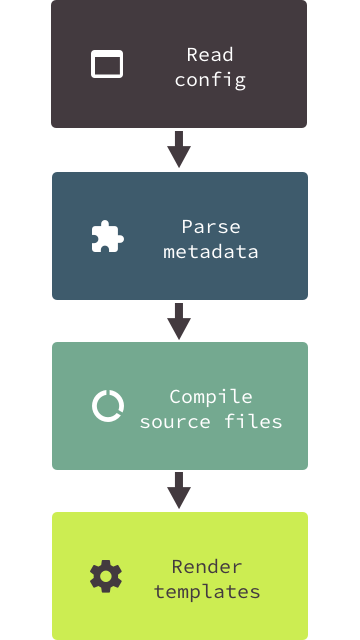
\includegraphics[width=0.9\textwidth]{build_pipeline.png}
    \caption{A graphic showing the basic flow of a \emph{build pipeline}.\\
    First, the configuration file is read and necessary modules invoked. Second, the global metadata, as well as metadata from within the content, is parsed and stored in the global configuration. Third, the content sources get compiled into basic \emph{HTML} markup. Last, the compiled content gets rendered into predefined templates, to apply a given structure which is used commonly throughout the website.}
    \label{fig:build-pipeline}
\end{figure}
%

A static site generator mostly consists of a build pipeline, which handles the workflow needed for bringing the content into shape. This goes from setting the boundaries, determined by a configuration file, to finally producing a web root, consisting of HTML, CSS and JavaScript files, as well as images.

Normally, the major part of it happens sequentially, as nearly all content files are facing a series of transformations on them \cite{Metalsmith2015technicaldocumentation}. Although the amount and extent of conversions may differ significantly from pipeline setup to pipeline setup, it can be broken down to the following core parts (see Fig. \ref{fig:build-pipeline}):

\begin{description}
  \item[Metadata parser] -- Parses global metadata, found in the configuration file or in the YAML frontmatter of content files.
  \item[Markdown compiler] -- Used to convert easily read- and writeable Markdown files in browser-readable HTML.
  \item[Template renderer] -- Responsible for bringing the very basic content structure in shape. The goal should be a common appearence, enriched with additional elements (like navigation, breadcrumbs, \ldots).
\end{description}

Of course, the list above overlaps at some point with the list mentioned in <<\emph{\nameref{par:creatingcontent}}>> on p. \pageref{par:creatingcontent}, as I consider a build pipeline just as a part of the given static site generator (although the main part), not as the generator itself. One of the reasons is its independence of programming languages: A build pipeline doesn't care which programming language it consists of, as long as it knows how to interpret the content sources and templates. Therefore, I may call it merely a concept, not a framework.

%% Say something about the config file, yadda yadda yadda one hand pure build pipeline, because of metadata and configuration, other hand no, because of plugins. plugins??

\subsection{Frontmatter}
\label{sec:buildpipelines-frontmatter}

\lstinputlisting[caption={frontmatter.md}, label={list:frontmatter}]{chapters/03-technical-foundations/_support/frontmatter.md}

listing \ref{list:frontmatter} shows a sample usage of frontmatter inside a Markdown file. Bounded by three dashes above the main content source, it allows certain per-file metadata definitions, which will be parsed at build time and provided for the template rendering engine.
% Mention something about omitting databases using frontmatter meta

As an example, the selected template for this sample file may also hold a list for the mentioned \emph{tags}, as well as a placeholder for the \emph{author}'s name and/or \emph{title}. The main content gets then rendered into the respective placeholding tag, already self-containing a basic structure.

Using a \emph{template: false} declaration, some plugins may prevent rendering the content into a template. This might be interesting in cases, where different partials should be included in the DOM by some sort of asynchronous JavaScript later on.


% TODO: Ugly, remove if not necessary anymore, cares for vertical spaces above subsections
\vspace{20pt}

\subsection{Markdown}
\label{sec:buildpipelines-markdown}

\lstinputlisting[caption={markdown.md}, label={list:markdown-demo}]{chapters/03-technical-foundations/_support/markdown.md}

\texttt{Markdown} consists of shorthand conventions, which should be easier to type for content creators  \cite[38]{dhillon2016}.
Therefore, it makes understanding \texttt{HTML} not a necessary precondition anymore, as a basic content structure may be easily achieved when prepending/surrounding text with certain special characters like \texttt{\#, *, \_, \ldots} (See Listing \ref{list:markdown-demo}).

Originally created by \emph{John Gruber}\footnote{\url{http://daringfireball.net/projects/markdown/} -- Markdown website.} as a plugin for \emph{Movable Type} and \emph{Blosxom} blogging engines \cite{Markdown2004introduction} in March 2004, it should be a supportive tool for users against the complexity of formal markup languages (e.g. \texttt{HTML5}) \cite[4]{RFC7764}. According to \emph{Gruber's} intention, there is no ``invalid'' \texttt{Markdown}, as he suggests the author should either ``keep on experimenting'' or ``change the processor'', if the output happens to fail his/her expectations \cite[5]{RFC7764}.

\texttt{GitHub} finally adapted \texttt{Markdown} to its own version, called ``GitHub Flavored Markdown'' (\emph{GFM}). The people behind it enhanced its original functions to also support \emph{code blocks, tables, strike-through text}, as well as \emph{auto-linking} URL structures in the content \cite[18]{RFC7764}. Additionally, also \texttt{GitHub}-specific functions, such as \emph{user mentions, commit references} or \emph{emojis}, may be used\footnote{\url{https://guides.github.com/features/mastering-markdown/\#GitHub-flavored-markdown} -- GitHub Flavored Markdown cheat sheet on \texttt{GitHub}.}.

Since then, \texttt{GitHub} renders browser-friendly versions of general descriptions written in \texttt{Markdown}, for providing fast and easy overviews of the respective repository. As an example, an existing \texttt{README.md} always appears below the root file tree section on a repository front page \cite[5]{gandrud2013github}.


% TODO: Ugly, remove if not necessary anymore, cares for vertical spaces above subsections
\vspace{20pt}

\subsection{Templates}
\label{sec:buildpipelines-templates}

\emph{Templates} are the frames of each content page, caring for a common, browser-readable HTML structure. A uniform design layout allows site-wide look and feel using a global CSS style sheet, as well as certain events triggered by user behaviour, handled by a single JavaScript file.

Born out of the need to fail-safe produce HTML on the server, as the produced data chunks -- initiated by a client HTTP request -- steadily grew, the goal behind templating engines is primarily to separate business logic from data display. Ideally, at the end of the day, there should be no code in HTML, and no HTML in code \cite[225]{Parr2004templates}.

\begin{program}
  \caption{post.hbs}
  \label{list:handlebars}
\lstinputlisting[language=HTML]{chapters/03-technical-foundations/_support/post.html}
\end{program}

A simple template file example for a blog post is shown in Program \ref{list:handlebars}. It is written in \emph{Handlebars}, a very basic templating language, offering only a very limited amount of template logic. Included are \emph{loops, if/else, partials,~\ldots}~--~however, additional ``\emph{helper}''-functions may be added by the developer.

Although such template logic may come in handy for the most part, as some business logic decisions seem to be rather taken during rendering, instead of being hard-coded before, the concept of data separation is therefore often unknowingly violated \cite[228]{Parr2004templates}. Thus, the choice of the ``optimal'' templating engine for a given project is crucial, as different engines offer a different range of built-in logic. This could go from very conservative \emph{Mustache}\footnote{\url{https://mustache.github.io/} -- Mustache website.} to very powerful ones like \emph{Liquid}\footnote{\url{https://help.shopify.com/themes/liquid} -- Shopify's Liquid template engine.} (see Sec. \ref{sec:jekyll-technology}) or \texttt{EJS}\footnote{\url{http://www.embeddedjs.com/} -- Embedded JavaScript website}.


\section{Git}
\label{sec:git}

Today, hardly any software project is started without any form of version control system (\texttt{VCS}). It supports developers as a back-up system and living archive of their work, as data generally is ephemeral and can be lost easily \cite[1]{loeliger2012version}. Although there are many different variations offered, some of the most popular today are \emph{Git, Apache Subversion, Mercurial} and \emph{Bazaar}.

\subsection{History}
\label{sec:git-history}
\texttt{Git} was initially published by \emph{Linus Torvalds} on April 7\textsuperscript{th}, 2005 \cite[6]{loeliger2012version}. This was necessary, as the ``free'' version of the then used VCS for the \emph{Linux} kernel development, \texttt{BitKeeper}, was restricted in a way it was not suitable any longer for the community behind it. Furthermore, the search of an already available alternative to the \texttt{BitKeeper} system failed due to an unsatisfying combination of needed features, so \emph{Torvalds} came up with his own VCS flavor, containing all desired functionalities for further \emph{Linux} development (among others) \cite[4]{loeliger2012version}:

\begin{itemize}
  \item Distributed development
  \item Handle thousands of developers
  \item Efficient performance
  \item Support branched development
  \item Free, as in freedom
\end{itemize}

While it was merely a tool for kernel hackers in the beginning, its simplicity quickly made developers use it for other projects too. However, the CLI still scared off people with less programming background, until \texttt{GitHub} came and introduced its Desktop client\footnote{\url{https://desktop.github.com/} -- GitHub Desktop client.}. Today, it is one of many GUIs, which are available for different operating systems\footnote{\url{https://git-scm.com/downloads/guis} -- Git GUI clients on the \texttt{Git} website.} and completely omits the necessity of terminal emulator knowledge when working with \texttt{Git}.

%% Write something, why it is so famous. distributed development - other use cases .. blargh.

\subsection{Technology}
\label{sec:git-technology}
Having decided to use \texttt{Git} as VCS, everything begins with setting up a new respository. This can be made remotely on a service like \texttt{GitHub}, or locally using \texttt{git init}. When initialized a local repository, it can still be published remotely through setting the correct URL using \texttt{git remote} later on \cite[198]{loeliger2012version}.

\subsubsection{Commits}
The next step would be working with the repository. For the most part, this should not influence the developer's workflow in any way, as the \texttt{.git} directory should be automatically hidden in most modern editors to not distract him/herself from the actual work. If the developer succeeded in a sub-task or simply wanted to save the current project state, he/she would create a \emph{commit}.

A \emph{commit} is a snapshot of the current repository's state. While it does not contain a copy of every file and directory in the project tree, it rather compares the current condition with its predecessing snapshot and creates a list of affected files and their changes. Blobs\footnote{\emph{BLOB} -- Binary Large OBject, a file which does not consist of queryable source code.} are either reused, if they remain unchanged or created new, if they were altered\cite[65]{loeliger2012version}.

Every \emph{commit} is organized in a way, that it is chained to its predecessor (\emph{parent}), thus representing a singly linked list with the ability of gaplessly going back from the current state (\emph{head}) to the initial \emph{commit} \cite[204]{dhillon2016}\cite[65]{loeliger2012version}. This is necessary, as it may happen to fix a bug or improve a design decision only by reworking a certain snapshot in the past \cite[151]{loeliger2012version}.

\subsubsection{Branches}

%% Graphic of git branches
\begin{figure} % h-ere, t-op, b-ottom, p-age
    \centering
    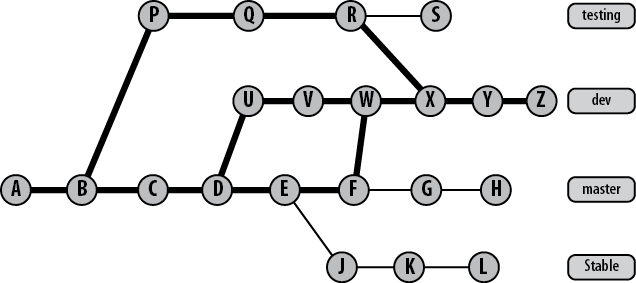
\includegraphics[width=0.8\textwidth]{git-branches.png}
    \caption{A graphic showing the basic structure of branches in \texttt{Git}.\\
    The \textbf{testing} branch was created out of project state ``B'', whereas \textbf{dev} was branched away from state ``D'' and currently holds the \emph{head commit} at ``Z''. In the meantime, \textbf{testing} was merged into \textbf{dev} at state ``R''. In the end, \textbf{dev} contains the commit history of all states connected with the bold line \cite[p. 92f]{loeliger2012version}.}
    \label{fig:git-branches}
\end{figure}
%

Since its early days, \texttt{Git} was used not only as back-up or archive system, but also as code management system. This is possible due to built-in functions, such as the so-called \emph{branched development}, where a current state of the actual development is duplicated and worked on separately. It allows for development to continue in multiple directions simultaneously \cite[89]{loeliger2012version} (see Fig. \ref{fig:git-branches}).

When being part of a remote team, a developer may also \emph{push} his/her own local branches for providing it to others, as well as keeping them for local development and \emph{merging} them back to the main branch after succeeding in his current task \cite[207]{dhillon2016}. Through the use of these possibilities, a responsible administrator keeping track of the development structure is not necessarily required to be appointed in any repository settings. Furthermore, the team may decide members in charge for merges in an agile way, based on the current need.

\subsubsection{Usage in static site development}
The advantages of using \texttt{Git} in static site development are mainly its possibilities of providing a full-featured archive of the content and source code of each project. Seamlessly going back and forth in the website development history makes it easy to navigate between every single content edit, without loosing track of previous and future revisions. In this case, it may work significantly better than using a common database system for content storage.

Furthermore, it is also possible to make use of \texttt{Git} \emph{hooks}. Once a new \emph{commit} is created, a \emph{hook} might take care of invoking the \textbf{build pipeline} as a ``post-receive'' \emph{hook} -- thus, the new website version gets built automatically without requiring any additional user interaction. However, \emph{hooks} should be only used with caution, as they are not distributed the same way as the files tracked in a given repository and also may harm the integrity of their \texttt{Git} repository \cite[p. 285f]{loeliger2012version}.

\section{GitHub}
\label{sec:git-github}

Already mentioned it a few times before (see p. \pageref{sec:jekyll}, \pageref{sec:buildpipelines-markdown} or \pageref{sec:git}), \emph{GitHub} is currently probably the most popular online collaboration platform, hosting not only the source code for the Linux kernel\footnote{\url{https://github.com/torvalds/linux} -- Linux kernel repository on GitHub.}, but also for other huge projects like Google's \emph{TensorFlow}\footnote{\url{https://github.com/tensorflow/tensorflow} -- Tensorflow repository on GitHub.}, Microsoft's \emph{.NET}\footnote{\url{https://github.com/Microsoft/dotnet} -- .NET repository on GitHub.} or Facebook's \emph{React}\footnote{\url{https://github.com/facebook/react} -- React repository on GitHub.}.

\subsection{History}
Tom Preston-Werner, a Ruby programmer from San Francisco and creator of earlier mentioned Jekyll (see ch. \ref{sec:jekyll} on p. \pageref{sec:jekyll}) and \emph{Chris Wanstrath} started developing GitHub in October 2007. After releasing a private beta in January, they released the site to the public on April 10\textsuperscript{th}, 2008 \cite{PrestonWerner2008githublaunch}.

Since then, GitHub grew very fast and quickly gained on popularity throughout the developer landscape, hosting more than 56 million projects today\footnote{\url{https://github.com/about} -- GitHub's ``about'' page.}. Thanks to their generous freemium pricing model, collaborating in open source projects still is for free: A free tier account may hold unlimited open source repositories, working together with unlimited contributors\footnote{\url{https://github.com/pricing} -- GitHub's pricing page.}. All in all it seems, that GitHub turned coding into a truly social activity \cite[416]{loeliger2012version}.

\subsection{Technology}
The main use case for creating a repository on GitHub is the fact, that unlike other privately hosted remote repositories, it offers a wide range of additional services. Services like \emph{Issue tracking, Pull requests} and \emph{Code reviews} leverage the maintainability of source code in a repository, making it easy for each developer to discuss and manage the current project state without the need of switching to a third party application.

%% Screenshot of GitHub in-page editor
\begin{figure} % h-ere, t-op, b-ottom, p-age
    \centering
    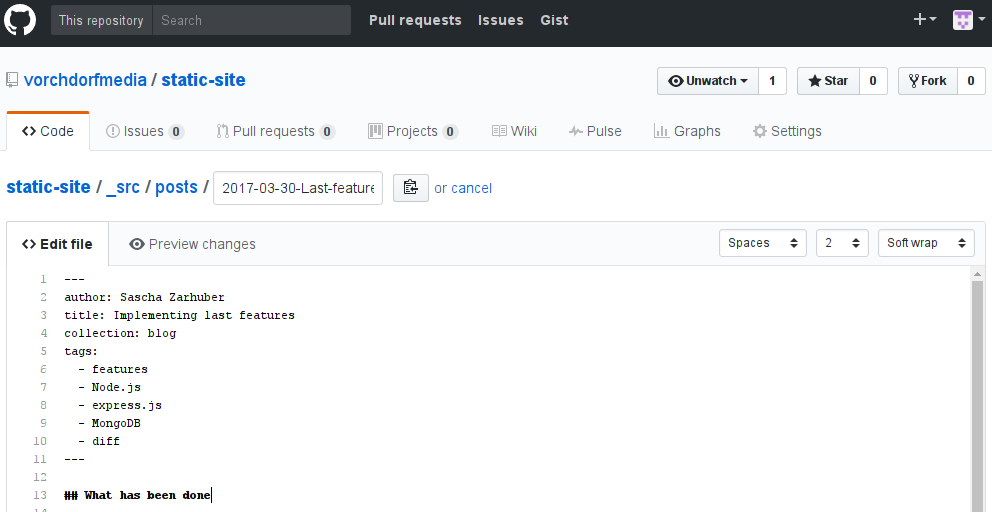
\includegraphics[width=0.9\textwidth]{github-page-editor.png}
    \caption{A Screenshot showing the \emph{In-Page Code Editor} of GitHub. An existing file is selected and ready to be edited. When finished, the user may commit the changes into the repository, so that other contributors also benefit from his/her adjustments.}
    \label{fig:github-page-editor}
\end{figure}
%

Especially for content authors without programming knowledge, the \emph{In-Page Code Editor} might be a very supportive tool, as it provides a clean and easy-to-use frontend for directly adding content to the repository (see Fig. \ref{fig:github-page-editor}). Additionally, the just edited file may not only be committed into the currently selected branch, but also in a newly created branch. Therefore, the source branch stays clean, whereas the edited file may get reviewed by an assigned supervisor, before being ready to get merged.\\
Furthermore, also developers might make use of this feature, especially when a small hotfix is to be made, where it would be too time-consuming to \emph{pull, commit} and \emph{push} from/to the repository \cite[405]{loeliger2012version}.

Pushing to a \emph{gh-pages} branch, or creating a \emph{<username>.github.io} repository, enables the use of GitHub's built-in website hosting service. From there, either a Jekyll project is freshly built, or already compiled static HTML are automatically published to the web -- additionally, custom domains may be used when adding a \texttt{CNAME} file \cite[p. 171f]{dhillon2016}.

\subsection{REST API}
Another significant advantage is the access of GitHub's REST API. Currently existing in its third major release, it almost offers every feature also available graphically in its web interface, as an equivalent JavaScript Object Notation (\emph{JSON}) upon programmatical request. Some services even feature more advanced data through the API than through the UI \cite[410]{loeliger2012version}.

When having the need of including data from a GitHub account into a third party service, a single authenticated HTTP request does the trick. Due to many available endpoints, a developer may quickly find the type information he/she needs to further process data directly from a repository. As an example, a complete listing of a repository's file tree is also possible, without needing to download and unpack an archive file. For one thing, this saves quite some time, for another thing, the requested data is already processed and presented, so that not only file paths are unveiled, but also their direct links and data types.

Furthermore, the API not only offers access to informational data about a given repository, instead, its manipulation through creating commits or uploading a file may also happen. To sum this up, very well documented examples are available on the API page on GitHub, where developers catch a good glimpse, of what is possible overall\footnote{\url{https://developer.github.com/v3/} -- API v3 documentation on GitHub.} \cite[401]{loeliger2012version}.


\section{GitHub}
\label{sec:git-github}

Already mentioned it a few times before (see p. \pageref{sec:jekyll}, \pageref{sec:buildpipelines-markdown} or \pageref{sec:git}), \emph{GitHub} is currently probably the most popular online collaboration platform, hosting not only the source code for the Linux kernel\footnote{\url{https://github.com/torvalds/linux} -- Linux kernel repository on GitHub.}, but also for other huge projects like Google's \emph{TensorFlow}\footnote{\url{https://github.com/tensorflow/tensorflow} -- Tensorflow repository on GitHub.}, Microsoft's \emph{.NET}\footnote{\url{https://github.com/Microsoft/dotnet} -- .NET repository on GitHub.} or Facebook's \emph{React}\footnote{\url{https://github.com/facebook/react} -- React repository on GitHub.}.

\subsection{History}
Tom Preston-Werner, a Ruby programmer from San Francisco and creator of earlier mentioned Jekyll (see ch. \ref{sec:jekyll} on p. \pageref{sec:jekyll}) and \emph{Chris Wanstrath} started developing GitHub in October 2007. After releasing a private beta in January, they released the site to the public on April 10\textsuperscript{th}, 2008 \cite{PrestonWerner2008githublaunch}.

Since then, GitHub grew very fast and quickly gained on popularity throughout the developer landscape, hosting more than 56 million projects today\footnote{\url{https://github.com/about} -- GitHub's ``about'' page.}. Thanks to their generous freemium pricing model, collaborating in open source projects still is for free: A free tier account may hold unlimited open source repositories, working together with unlimited contributors\footnote{\url{https://github.com/pricing} -- GitHub's pricing page.}. All in all it seems, that GitHub turned coding into a truly social activity \cite[416]{loeliger2012version}.

\subsection{Technology}
The main use case for creating a repository on GitHub is the fact, that unlike other privately hosted remote repositories, it offers a wide range of additional services. Services like \emph{Issue tracking, Pull requests} and \emph{Code reviews} leverage the maintainability of source code in a repository, making it easy for each developer to discuss and manage the current project state without the need of switching to a third party application.

%% Screenshot of GitHub in-page editor
\begin{figure} % h-ere, t-op, b-ottom, p-age
    \centering
    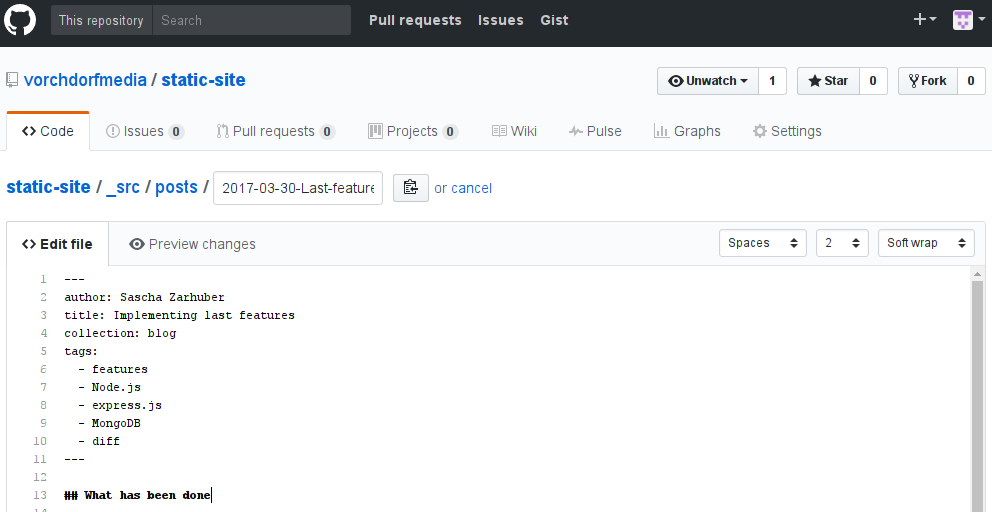
\includegraphics[width=0.9\textwidth]{github-page-editor.png}
    \caption{A Screenshot showing the \emph{In-Page Code Editor} of GitHub. An existing file is selected and ready to be edited. When finished, the user may commit the changes into the repository, so that other contributors also benefit from his/her adjustments.}
    \label{fig:github-page-editor}
\end{figure}
%

Especially for content authors without programming knowledge, the \emph{In-Page Code Editor} might be a very supportive tool, as it provides a clean and easy-to-use frontend for directly adding content to the repository (see Fig. \ref{fig:github-page-editor}). Additionally, the just edited file may not only be committed into the currently selected branch, but also in a newly created branch. Therefore, the source branch stays clean, whereas the edited file may get reviewed by an assigned supervisor, before being ready to get merged.\\
Furthermore, also developers might make use of this feature, especially when a small hotfix is to be made, where it would be too time-consuming to \emph{pull, commit} and \emph{push} from/to the repository \cite[405]{loeliger2012version}.

Pushing to a \emph{gh-pages} branch, or creating a \emph{<username>.github.io} repository, enables the use of GitHub's built-in website hosting service. From there, either a Jekyll project is freshly built, or already compiled static HTML are automatically published to the web -- additionally, custom domains may be used when adding a \texttt{CNAME} file \cite[p. 171f]{dhillon2016}.

\subsection{REST API}
Another significant advantage is the access of GitHub's REST API. Currently existing in its third major release, it almost offers every feature also available graphically in its web interface, as an equivalent JavaScript Object Notation (\emph{JSON}) upon programmatical request. Some services even feature more advanced data through the API than through the UI \cite[410]{loeliger2012version}.

When having the need of including data from a GitHub account into a third party service, a single authenticated HTTP request does the trick. Due to many available endpoints, a developer may quickly find the type information he/she needs to further process data directly from a repository. As an example, a complete listing of a repository's file tree is also possible, without needing to download and unpack an archive file. For one thing, this saves quite some time, for another thing, the requested data is already processed and presented, so that not only file paths are unveiled, but also their direct links and data types.

Furthermore, the API not only offers access to informational data about a given repository, instead, its manipulation through creating commits or uploading a file may also happen. To sum this up, very well documented examples are available on the API page on GitHub, where developers catch a good glimpse, of what is possible overall\footnote{\url{https://developer.github.com/v3/} -- API v3 documentation on GitHub.} \cite[401]{loeliger2012version}.

\section{Diff}
\label{sec:diff}

``\emph{diff} reports file differences between two files, expressed as a minimal list of line changes (\ldots)'' \cite[1]{Hunt1976}. Existing more than 40 years now, it has been an essential tool for file comparison throughout the history of computing -- furthermore, it is also a core component of Git, which contains its own version called \emph{git diff} \cite[108]{loeliger2012version}.

\subsection{History}
\label{sec:diff-history}
Initially published by \emph{James W. Hunt} and \emph{Malcolm D. McIlroy} in July 1976 when working at \emph{Bell Labs}, the algorithm was later used in \emph{UNIX} as application called diff. \emph{Paul Eggert} and \emph{Richard Stallman} (among others) also wrote the diff application as part of their \emph{GNU diffutils}\footnote{\url{http://manpages.ubuntu.com/manpages/zesty/en/man1/diff.1.html} -- Manpage for GNU diff.}, which is nowadays mainly distributed in Linux derivatives, MacOS, as well as part of Git. They used an improved algorithm published by \emph{Webb Miller} and \emph{Eugene W. Myers} in 1985 \cite[3]{mackenzie2003comparing}, who proved, that the original ``Hunt-McIlroy algorithm'' is inefficient on certain special cases. As a test case, they used a file containing 1000 blank lines, and a second file, consisting of the initial file, but containing a single non-blank file on both ends. As a fact, using other experiments performed on typical files, Miller's and Myers' algorithm ran roughly four times faster \cite[p. 1034f]{miller1985file}.

\subsection{Technology}
\label{sec:diff-technology}

\begin{lstlisting}[label={list:diff-normalformat}, caption=sample.diff]
0a1
> w
3,4c4,6
< c
< d
---
> x
> y
> z
6,7d7
< f
< g
\end{lstlisting}

diff's core task is finding the ``shortest sequence of insertions and deletions that will convert the first string to the second'' \cite[1025]{miller1985file} together with finding the longest common subsequence occurring in both files \cite[2]{Hunt1976}. Combined with the mathematical algorithm, it should provide an easily understandable format for humans, consisting of line numbers joined with \emph{a, c} or \emph{d} (append, change, delete), as well as \emph{<} and \emph{>} line prefixes, showing the affiliation either to the initial or compared file. This is called the ``Normal Format'' \cite[12]{mackenzie2003comparing}. Listing \ref{list:diff-normalformat} shows a sample output, comparing the strings \texttt{a b c d e f g} and \texttt{w a b x y z e} (one line per letter)\cite[p. 1f]{Hunt1976}.


% TODO: Ugly, remove if not necessary anymore, cares for vertical spaces above subsections
\vspace{20pt}
\subsubsection{The Unified Format}

To provide a more readable user experience, GNU diff contains an improved format, called Unified Format, removing redundancy by using a more compact syntax. It can be selected as output format by executing diff together with a \texttt{-u} flag \cite[16]{mackenzie2003comparing}, whereas git diff uses this as standard format to show changes within the current working tree \cite{GitDiff}.


\begin{lstlisting}[label={list:diff-unifiedformat}, caption=unified\_format.diff]
--- oldfile	2017-04-13 09:42:47.474769553 +0200
+++ newfile	2017-04-13 09:43:13.898566935 +0200
@@ -1,7 +1,7 @@
+w
 a
 b
-c
-d
+x
+y
+z
 e
-f
-g
\end{lstlisting}

As an example, listing \ref{list:diff-unifiedformat} shows the same diff output as listing \ref{list:diff-normalformat}, only as Unified Format using the following components:

\begin{description}
  \item[\texttt{------ \{filename\} \{timestamp\}}] -- indicates the initial file together with the timestamp it was created,
  \item[\texttt{+++ \{filename\} \{timestamp\}}] -- same as above, but for the compared file
  \item[\texttt{@@ -\{intial line range\} +\{compared line range\} @@}] -- \texttt{-1,7} indicates the following 7 lines, starting from the first line of the initial file
  \item[\texttt{+}] -- marks a line as added in compared file
  \item[\texttt{-}] -- marks a line as deleted in compared file
\end{description}

To make the above explanation a little bit more clear, an additional example with a text speaking for itself is added below:

\lstinputlisting[caption={file.diff}, label={list:diff-explanation}]{chapters/03-technical-foundations/_support/file.txt}

It can be clearly seen, that line 3 shows a growth of \emph{newfile} by two lines: -1,8 vs. +1,10. Having also a color-coded representation, it would boost the readability of such diff outputs once again.


% TODO: Ugly, remove if not necessary anymore, cares for vertical spaces above subsections
%\vspace{20pt}
\subsubsection{Usage with Git}
As already stated, diff is one of the core components of Git. Not only does it support determining changes in the source code between a snapshot and another, it may also reveal merge conflicts, if segments are mutually exclusive and therefore preventing a flawless propagation of development. Thus, a varying development history of different origins (e.g. branches) not compatible to each other might be indicated. Furthermore, a conflict may also happen, if a developer forgot to \emph{pull} the latest changes before committing his/her current development progress. These conflicts may only be handled through human guidance \cite[124]{loeliger2012version}.

\begin{lstlisting}[label={list:diff-conflict}, caption={A snippet of a file called ``manual.txt'', which is affected by a conflict. Content between \texttt{HEAD} and \texttt{=======} contains the local version, content below contains the foreign conflicting version.}]
<<<<<<< HEAD:manual.txt
I (the developer) am right!
=======
The branch_name is right!
>>>>>>> branch_name:manual.txt
\end{lstlisting}

A conflict presents itself primarily through a message similar to:\\
\texttt{CONFLICT (content): Merge conflict in file\\
Automatic merge failed; fix conflicts and then commit the result.}\\
If anything like the above happens, the affected files by the conflict also contain a structure like shown in listing \ref{list:diff-conflict}. A conflict can then be resolved by removing its markers and picking the appropriate resolution of either side of the \texttt{=======} delimiter \cite{GitConflicts}, as well as mixing them to the developers needs \cite[126]{loeliger2012version}. A single file may also contain multiple conflicts.

\subsubsection{Usage with GitHub}
Especially when interacting with GitHub's REST API, it is very easy to generate and import file diffs of a given repository. Whether two branches or two commits using their \emph{SHA} values are compared, a single HTTP request suffices for programmatically retrieving data, which is normally only accessible using a terminal emulator.

Depending on the requested \emph{media type} in the appropriate HTTP header field, either a full-featured diff, patch or JSON containing per-file patches is emitted by the API. If the latter was used, the underlying diff is translated into a JSON object, containing information like the number of additions, deletions and changes, as well as the mentioned \emph{patch} for each file.

As a consequence, a repository does not necessarily have to be \emph{cloned}, as it may be patched constantly using the API to keep it up to date -- using this method, patch is even able to create and delete files, if necessary \cite[57]{mackenzie2003comparing}. The only prerequisite is to keep track of the single commit hashes the patches are applied from.


\chapter{Theoretical approach}
\label{cha:theoreticalapproach}

Once a decision is made in favor of a project using a static site generator, first challenges may already arise:

\begin{itemize}
  \item What kind of media is being used? Images, videos, or just text?
  \item How is the project structured? How many independent permalink structures are there?
  \item How many content authors are there? How often is content added or altered?
  \item How steady is the site design? Does the site have more than one independent design flow?
\end{itemize}

Some issues described by one or more of the questions above may not be improved in a predictable amount of time. Some of them are mostly content-related, others are related to development. Even in projects where only a high amount of content productivity is pursued, developers are forced to keep the build pipeline performant and responsive to the content author's needs.

\section{Challenges}
\label{sec:challenges}

As already stated above in the introduction, nearly every web project bears challenges to solve, both for developers on the one hand, and for content creators on the other hand. While content creators mostly need to solve structural issues in the published content, developers are mainly responsible for supporting authors in technical questions, as well as constantly keeping an eye on the backend development. This might go from always keeping the underlying modules updated, to populating the source code with design or template changes, to finally maintaining the build pipeline and deployment setup.

\subsection{Distributed development}
\label{sec:challenges-distributeddevelopment}

When it comes to administer a static site project, it is very likely, that there will not be any possiblity of working on the same project in the same environment in a linear way. Instead, every developer will have to have a local install of the used generator at his/her disposal, together with access to a remote repository of a version control system for exchanging the current development process with other project maintainers. The main reason for that is the fact, that unlike content authors, developers do have the obligation of installing or maintaining the project's dependencies \cite[85]{dhillon2016}, thus not only for testing reasons.

If using GitHub for example, content editors, on the other hand, may easily make use of the built-in ``In-Page Code Editor'' (see Fig. \ref{fig:github-page-editor} on p. \pageref{fig:github-page-editor}), which also provides an optimistically rendered version of the current content, although without making use of the project's style sheet.

%% Graphic of separating project repositories
\begin{figure} % h-ere, t-op, b-ottom, p-age
    \centering
    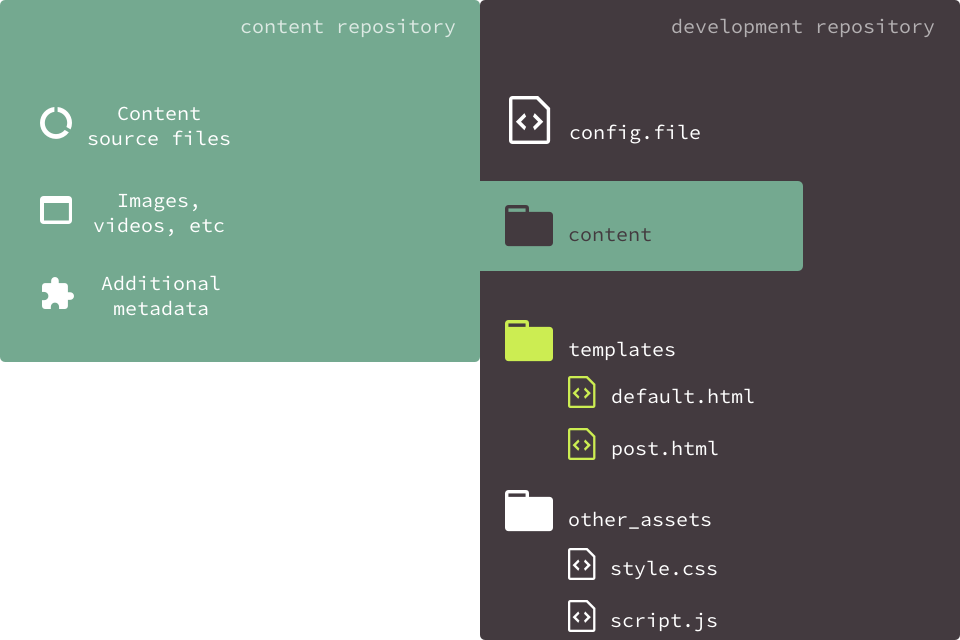
\includegraphics[width=0.9\textwidth]{challenges-repositories.png}
    \caption{A graphic showing the stylized separation of a project into a \emph{content} and a \emph{development} repository. The content authors may only be granted access to the content repository, while developers should be granted access to both, thus providing a seamless integration for the content into the build pipeline flow (see Fig. \ref{fig:build-pipeline} on p. \pageref{fig:build-pipeline}).}
    \label{fig:repository-separation}
\end{figure}
%

\subsubsection{Separating content from code}
As constantly growing static site projects may sooner or later come to a point, where content progression differs from development progression, it might be useful to separate both parts into independent repositories (see Fig. \ref{fig:repository-separation}). This especially makes sense, if the content editor team is also separated from the development team and therefore an additional level of security against accidental branch intermixture is needed.

\subsubsection{Merging only using pull requests}
However, if this kind of strong division is not desired anyhow, another option would be to limit access to the development repository in a way, that everyone may \emph{fork} a repository, but only certain project users are allowed to \emph{merge} external branches into the main development tree. On GitHub, \emph{pull requests} may be used. These pull requests allow any user to announce his/her contribution to the project using a commit history of a forked repository. The source project owners may then decide whether or not to merge the announced changes and also have the chance to express their point of view via comments directly on the pull request to its creator \cite[p. 394f]{loeliger2012version}.

The point in time a pull request is created is although subsidiary, as further development on the specific branch is as well automatically included, as per-line comments are also removed, once the specific line of code has been modified in a following commit \cite{GithubPullRequests}. Furthermore, the possibility to merge is checked after every commit pushed to the respective branch, so the responsible users always know, if a merge operation may be successfully executed before being able to complete the process by clicking the green ``Merge pull request'' button. Otherwise, a merge is only possible after locally checking out the pull request and processing it via the command line \cite{GithubMergePullRequests}.

\subsubsection{Staging versions}
Working with separate remote branches on a version control system like Git also allows for staging environments and therefore testing out different versions of the projects concurrently. The public version however, visible to all clients visiting the website, remains the most stable and might receive only well-tested or well-considered updates as the very last step in the ongoing development.

To achieve this goal, a testbed is necessary and may be realized using another branch besides ``master''. Sometimes an additional ``bleeding edge'' version is also likely to be included in the build process. Based on this strategy, it is easy to control and maintain different revisions at the same time and nevertheless infer the functionality of different proof of concepts for merging them into the public version later on.


\subsection{Build cycle completion}
\label{sec:challenges-buildcyclecompletion}

One of the major challenges remains the issue of providing a ``real website look and feel'' to the content editor. Whereas authors in dynamic CMSs are presented with an already pre-rendered version of the newly added content (since the underlying system is not dependent on any template rendering before deployment), static site generators first offer a glance of the author's work, after the whole build pipeline process succeeded in its render flow, unless other pre-caching methods are used. Yet, most static site generators do not include such kind of tools by default.

Based on the size and the amount of files in the website source code, this time frame can easily grow linearly. If there are also additional tasks added to the build process, such as resizing images to different screen sizes for providing a  responsive user experience, the computational effort may easily get out of hand and therefore the duration until the content editor first sees the result of his/her work simply gets unacceptable.

\subsubsection{Possible problems of long-lasting build processes}
Waiting for the completion of the build pipeline can cause severe recesses in the work performance of a content editor or developer, as mostly any further work depends on its success, while a failure is often combined with time loss beforehand and intensive bug hunting afterwards -- probably resulting in even more consecutive build pipeline failures. This assertion may not only be linked to crucial modifications in development, also the smallest hotfixes might as well provoke a full rebuild without justifying the whole effort.

Furthermore, being forced to wait in line as a developer may cause him-/herself to loose track on the development process, thus the introduction of sustainable bugs (although not resulting in a build failure) is more likely. Additionally, mindlessly executing build cycles may even lead to data loss or blocking the workflow of other contributors.

%% Graphic of caching theory
\begin{figure} % h-ere, t-op, b-ottom, p-age
    \centering
    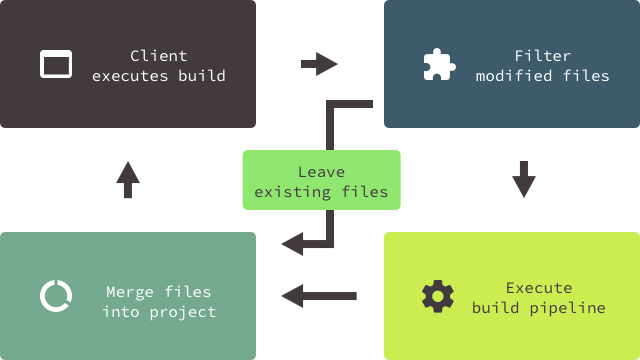
\includegraphics[width=0.9\textwidth]{challenges-caching.png}
    \caption{A graphic showing the theoretical approach of a build process flow, supported by caching.\\
    After the \emph{client} (content creator, developer) executes a build, the included caching mechanism should filter modified or added files and send them to the build pipeline. After the build succeeded, the newly built files should be merged with the already existing files to form an updated version of the website root.}
    \label{fig:caching}
\end{figure}
%

\subsubsection{Choosing an appropriate caching method}
Speeding up a build process can be done via \emph{caching}. The right caching method should differ between unmodified content and files which actually have been reworked or were newly introduced into the project source. Using this sort of information, the algorithm might only choose the latter files, send them to the build pipeline and assemble the outcome to the already existing project build (see Fig. \ref{fig:caching}).

Although a few static site generators already include some sort of caching methods -- although most of them only work locally (like Hexo's Warehouse, see ch. \ref{sec:hexo-technology}), a first step is made. It should significantly improve the build duration for local development, as long as the optimal cache storage is being used. Hexo's Warehouse uses a \emph{JSON} file as persistant storage, while the temporary storage lies in the Computer's RAM. This is fine for smaller projects, but could also lead to critical memory issues when used in projects containing a huge amount of files. For bigger data sets, it would be possible to use caching in conjunction with databases like \emph{SQLite} using the \emph{JSON1} extension\footnote{\url{https://www.sqlite.org/json1.html} -- JSON1 documentation on SQLite's website.}, however, the necessary effort at the beginning for providing a working mechanism should be well considered.

Nevertheless, a major issue still remains, as the local cache may not easily be transferred to other contributors or deployment engines, so that the first build after each pull does not take advantage of any speed up technique. Moreover, the methods mentioned above all use a significant amount of computing power to provide a useable cache, which could lead to problems and unwanted slowdowns on portable devices.

\subsubsection{Determination of cacheable contents}
When having overcome the decision and setup of the respective caching system, the next step would be to select cacheable files, as not every file has the same impact on the project source. While normal blog posts mostly belong to their own, unless there is probably a preview featured somewhere, a template file on the other hand, is often a dependency for many blog posts. Therefore, it can be said, that a working cache is more important for a commit only containing blog posts, than for a commit which only contains template files.

%% blargh -- dependency management, sitemap, etc...

\section{Solution strategies}
\label{sec:solution-strategies}

A primary task would be the focusing on critical issues to at least boosting the project's overall performance noticeably without losing too much track. This may be worked on in terms of collaboration, as well as in the project's setup, where on the one hand the team's performance and on the other hand the build engine's performance should be improved.

A lot of issues can be covered using GitHub's API, although some project specific adaptions are still necessary. Nevertheless, the API provides enough information for quickly perceiving a sufficient overview of the respective repository.


\subsection{Distributed development on GitHub}
\label{sec:solutions-distributeddevelopment}

Based on GitHub's API and the advantages of using Git as version control system, it is definitely a significant benefit to equip all project contributors with a GitHub account. While the public, open-source model is free of charge (see Sec. \ref{sec:github-history}), there are also different pricing models offered for privately held projects, which should be hidden to the public\footnote{\url{https://github.com/pricing} -- GitHub's pricing models.}.

Although dependent on financial expenditures, the additional value of working on a project with closed source (though it may be released as open source somewhere in the future) may be worth considering. Yet, full-featured access to the API is also included in the free tier though.

Not only GitHub offers a queryable API, also \emph{Bitbucket} provides an API with similar response data\footnote{\url{https://developer.atlassian.com/bitbucket/api/2/reference/} -- Bitbucket's API documentation.}, although certain features are missing, compared to GitHub. These missing features include for example certain project download functions, among others.

In addition to the API, GitHub's built-in In-Page Code Editor plays an important role for choosing it as core support tool for this project. Therefore, merging using pull requests and a continuous branching model for supporting staging versions qualify as proposed strategies to developers.


\subsection{Build cycles}
\label{sec:solutions-remotebuilding}

Supporting content authors in their workflow also means to not require them to install unnecessary build tools manually, unless critically needed. Due to the possibility of using GitHub's In-Page Editor, the whole Git checkout, commit and push process becomes in a way redundant too. Moreover, the online editor automatically creates pull requests on demand, so that the respective project owners should get notified automatically, if a merge is possible and therefore an update of the currently published project may be initiated.

Normally, a responsible user would pull the new state after a merge of the pull request, then execute the build pipeline. After the build process succeeded, he/she then has to take care for updating the webroot on the server, so that the newest version of the website gets delivered to the client upon request. However, this practice may easily get cumbersome, as the respective developer might get distracted by checking out new branches and possibly leaving behind his/her own work for the moment. Moreover, if the deployment has to be done manually, additional mistakes may happen during the whole action.

In this case, it makes sense to remotely outsource the build service and to possibly even automatically execute the render cycle. Used in conjunction with GitHub's \emph{Webhooks}, an external service would receive a build execution order via a HTTP POST request, based on certain predefined events in the GitHub repository \cite{GithubWebhooks}. Apart from the information the webhook provides, the service would even accept custom build options issued by responsible users, as the endpoint has to be publicly available anyhow. Once a build succeeds, the service should then notify a predefined list of users about the render cycle result and provide the outcome via download possibility.

\subsubsection{Existing remote services for static site generators}
\emph{CloudCannon}\footnote{\url{http://cloudcannon.com} -- CloudCannon, the Cloud CMS for Jekyll.} is probably the most popular online static site generator and offers a commercial external building service for Jekyll projects, together with source access using a GitHub or Bitbucket repository. According to its documentation, it currently supports Jekyll projects running v2.4.0 or newer\footnote{\url{https://docs.cloudcannon.com/building/versions/} -- Supported versions on CloudCannon documentation.}. It features a project file explorer and presents every new project as opinionated as Jekyll usually does (see Sec. \ref{sec:jekyll-technology}), as well as an automatic deployment service on their own subdomains. However, access to the rendered website files is not included, so every customer is dependent on using their hosting service.

\emph{BowTie}\footnote{\url{https://bowtie.io} -- Website of BowTie.} is similar to CloudCannon and is also offering a commercial online service. It seems to be a much more standalone service than CloudCannon, though it also offers GitHub integration, as well as custom Webhooks for event-based actions on external services.

%% Screenshot of Pancake push fail
\begin{figure} % h-ere, t-op, b-ottom, p-age
    \centering
    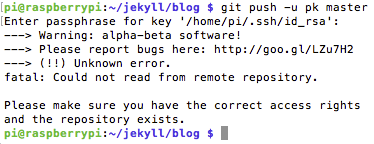
\includegraphics[width=0.75\textwidth]{remote-pancake.png}
    \caption{A screenshot of an approach to pushing a Jekyll project to \emph{Pancake}. As a result, the operation failed with an ``Unknown error''.}
    \label{fig:remote-pancake}
\end{figure}
%
\emph{Pancake}\footnote{\url{https://www.pancake.io} -- Website of Pancake.} is a free service for externally building static sites. It features an engine auto-detection and currently supports \emph{Jekyll, Wintersmith, Pelican, Sphinx, Hyde} and \emph{Middleman}\footnote{\url{https://github.com/pancakeio/detect/blob/master/heuristics.go} -- Currently supported static site generators by Pancake in raw source file on GitHub.}. Due to its non-commercial version, several restrictions are to be considered \cite{PancakeGitProjects}.

However, the service does currently not run stable, as an initial project setup failed (see Fig. \ref{fig:remote-pancake}). It seems that Pancake uses a post-receive hook for automatically trying to build a project, once it detected the underlying engine type. This causes waiting time for the developer on the one hand, but on the other hand informs whether a build was successful or failed. During another push attempt, it failed, as \emph{bundler}\footnote{\url{http://bundler.io} -- Bundler, a gem dependency manager.}, a gem dependency management tool required by Jekyll, was not mentioned in the ``Gemfile'' contained in the repository.

\subsection{Caching}
\label{sec:solutions-caching}

As stated before, most static site generators do not contain any form of caching mechanism by default -- if they do, caching is limited to the local machine a build is executed on. Since there is probably not an easy way of providing a form of remote caching, as this largely includes the necessity of external services to exchange a common status, as well as an index containing information about source and destination files for later rebuilds, it needs an equivalent strategy, which merely contains these information from a certain point in the past to the present, without relying on physical file structures to be exchanged.

Furthermore, such a caching strategy must be universally useable across all operating systems and ideally does not require any additional setup from the user. Moreover, it should also feature hassle-free integration into any project without depending on an external, yet unused service.

Keeping all of these issues under consideration, not every suggestion might get featured equally in the final solution -- the main reason is, that a kind of transformation like the one caused by a build pipeline always needs an existing status to build up from. So, tradeoffs are likely to accompany any form of decision to be made in this case.

\subsubsection{Caching based on diff}
As Git was chosen as version control system, diff is already part of the development suite. Therefore, a gapless detection of development progress between two arbitrary commits is possible. The diff format can be parsed to JSON and makes it easy for use in JavaScript. Thus, its usability for further processing on application level is assured\footnote{\url{https://runkit.com/saschazar21/diff-parsing-demo} -- An interactive example for fetching and parsing a diff-file.}.

The most important parts of a diff representation in this context are the file paths, as well as the type of modification on each file affected in the respective time span. Considering this kind of information, an existing repository might be quickly divided into unaffected and affected files -- where affected files, as well as their dependents possibly need to be selected for a rebuild. The final decision of the rebuild extent based on the diff, however, should be based on heuristics.

To conclude the consideration of using diff, the approach explained above is different from ``classical'' caching. Such a mechanism, founded on diff, is not dependent on support-files produced on its own (like a caching catalogue), but it requires a consistent and strict git workflow, otherwise it has no control over untracked files.

\section{Preparing for implementation}
\label{sec:primarythoughts}

After looking at challenges and possible solutions to them, a few keywords are essential:

\begin{description}
  \item[Remote] -- Outsorce long-lasting actions to an external service.
  \item[Cache] -- Speed up builds by making use of already finished work.
  \item[Versioning] -- Keep track on development and possibly revert, if necessary.
  \item[Branches] -- Let different parts of development evolve to their own speed.
\end{description}

While it may appear, that the above list is too fixated on version control systems, it should be clear now, that especially Git qualifies core companion to any website project, especially when the project itself is maintained by multiple developers, designers and/or authors. Being aware of GitHub as social code management tool and moreover the benefits of its API, the foundation stone should be laid (see ch. \ref{sec:solutions-distributeddevelopment} on p. \pageref{sec:solutions-distributeddevelopment}).

%% Graphic of basic api flow
\begin{figure} % h-ere, t-op, b-ottom, p-age
    \centering
    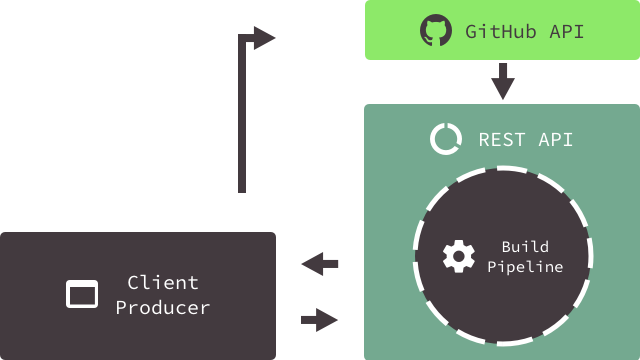
\includegraphics[width=0.75\textwidth]{api_flow.png}
    \caption{An abstract flow visualization of the planned request cycle. The client (developer, content creator) manages his/her code on GitHub. Based on the respective configuration, a build cycle may be triggered either using a GitHub webhook, or by manually sending a POST request to a certain endpoint.    That request then gets caught by the REST API, which creates an instance of the build pipeline. The pipeline requests data of the project from GitHub and sets up the project configuration. After a successful build, the REST API provides a downloadable archive of the newly built webroot.}
    \label{fig:api-flow}
\end{figure}
%

Since the tool should also be remotely accessible, it makes sense to also design it as RESTful API, for handling programmatical access as well as access from possible frontend apps lying on top. Furthermore, its main work cycle might get detached for neither distracting users due to ordering them to wait until it finished, nor blocking access in between (see Fig. \ref{fig:api-flow}).

However, the most important part behind these thoughts is the choice of the ideal static site generator.


\subsection{Choosing a static site generator}
\label{sec:primarythoughts-generator}

Due to the fact, that the choice of the best possible static site generator is the linchpin for a project like this, the evaluation needs to cover its usability, pluggability, customizability and overall maintenance, as well as the level of its general support. First and foremost, the installation process should be as easy as possible and not rely on too many third-party dependencies, which are probably not needed afterwards. Through this, it may be guaranteed, that also users, who are foreign to development, are likely to set up an instance on their local machines, although not critically required. This creates awareness for the project structure and therefore may lead to less support requests in the future.

The programming language of the chosen static site generator does have to be considered well, as it has to fit seamlessly into a planned REST API, in the best case without any further adapter in between. This should make it also easy to hook additional code into the configuration step, if needed. Ideally, it emits events as well, so any host process knows when a detached process is finished.

All in all, the best possible solution seems to be \emph{Metalsmith} (see ch. \ref{sec:metalsmith} on p. \pageref{sec:metalsmith}), as it not only offers a pluggable module ecosystem, but also access to a JavaScript API, among others. Together with some custom tweaks (e.g. dynamic module loading), an independent build setup for each project may be injected using only a specific configuration file.


\subsection{Constructing a REST API}
\label{sec:primarythoughts-restapi}

JavaScript proved its universality due to its usage both on client- and server-side, thus, a major advantage is its common knowledge among developers combined with a low barrier to entry for people, which are already found in frontend-development.

Node.js is a server-side implementation for JavaScript, backed by Google's V8 engine, which directly translates the scripting language into machine code \cite[4]{cantelon2017node}. This perfetly supports developers in reducing their tradeoff for possibly having to handle multiple ecosystems at once. A seamless integration of Metalsmith into the API service may therefore happen without much hassle.

The easy installation is supported by several third-party apps like Node Version Manager (\emph{NVM})\footnote{\url{https://github.com/creationix/nvm} -- NVM's repository on GitHub.} and mostly will not need any admin rights, which makes it ideal to use on hosting environments without root access (unlike PHP or Ruby for example). Although not equally well supported among the most popular operating systems, at least MacOS and Linux provide a stable enough environment for NVM.

Looking for a framework for setting up an API, \emph{Express}\footnote{\url{http://expressjs.com/} -- Website of Express.} seems to be the perfect fit, as it consists only of a very basic setup -- similar to Metalsmith -- but may be easily enhanced using different node modules, thus providing a uniquely shaped web application in contrast to conventional, monolithic frameworks like \emph{Django} or \emph{Ruby on Rails} \cite[176]{cantelon2017node}.

% Express sample basic configuration
\lstinputlisting[caption={An example for a basic express.js setup, roughly taken from \url{http://expressjs.com/en/starter/hello-world.html}.\\
In this case, a web application listens for a \emph{GET} request on its root path ``/'' and responds with a ``Hello World!'' message.}, label={list:express-setup}, language=JavaScript]{chapters/04-theoretical-approach/_support/express.js}

As a result, the main purpose of such an express application would be acting as a web-based infrastructure for the underlying build pipeline. Based on different REST endpoints, as well as their request parameters, executing a uniquely configured Metalsmith process on a project directory within the API's file tree should be possible without any further external interaction requirement. The project directory would be provided using an appropriate GitHub repository, requiring only a basic, as little opinionated configuration as possible, together with a public access possibility to the repo.

Additionally, to benefit most from any remote outsourcing, a current production-ready version of the project may be held available at a special endpoint for downloading at any time. In this case, further processing is enabled without waiting for completion of any build cycle beforehand, unless the source code received any updates through development.


\subsection{Selective rendering}
\label{sec:primarythoughts-rendering}

While the theoretical foundations for a project covering the use case of static site generation are now defined, a constantly growing amount of necessary build time still remains as one of the core problems. Caching across remote machines is likely to be impossible, especially if local computers also have to be added to the caching network and not every node is working on the same project revision at the same time. Moreover, an additional distribution mechanism would also have to be implemented, acting primarily as supply tool for providing already rendered revisions of different steps in development.

If cutting down on expectations and concentrating on basic improvements of speeding up a build cycle, a solution without exchanging complete file trees might be possible. To make sure all required data is accessible, the respective GitHub API credentials are mandatory. The main reason behind that is the gapless availability of every commit and its underlying file tree via HTTP -- therefore a separate \texttt{git checkout} on server level is not needed, GitHub provides the according file tree as immediately obtainable tarball or zip archive.

Together with the development history between two individual commits resulting in a diff and a downloadable file tree representing a certain step in the current progress, a build log has to keep track of the ongoing rendering actions and their results. The idea behind that is the possibility of remembering any render action in the past and incrementally building up on the latest positive result by only selecting the modified files for use in the build pipeline and leave out any other. Relying on an already available bugless result of a previous build cycle, any successful outcome of an upcoming action based on a later commit may be easily merged (see ch. \ref{sec:solutions-caching} on p. \pageref{sec:solutions-caching}).


\chapter{Implementation}
\label{cha:implementation}

After shaping a basic theoretical approach and probably sketching different considerations, it is time to define the needed tools and setting up a project repository. Also, it has to be considered, that the finished project should depend on as little third-party software as possible, but also be as deployable as possible.

At the very beginning, a clear structure has to be adopted, which concurrently serves as navigation guide for later development. Having a folder structure ready at development start, it may seem rigid and even narrow down the developer's freedom in creating his/her part of the application logic during some part of the process, but nevertheless it is definitely an important and easy supporting tool for projects being maintained using an asynchronous collaboration workflow. Furthermore, it may even help in creating tasks focusing on certain parts of the development process.

\section{Foundation}
\label{sec:foundation}

Since Node.js is very suitable for providing an instant development environment on most popular operating systems\footnote{\url{http://nodejs.org/dist/latest/} -- Precompiled versions of the latest Node.js release, for different operating systems.}, as well as quickly leveraging a basic application, which provides immediate feedback to its creator -- without depending on any precompilation steps -- it may be considered as basic framework for any further development.

Together with the achievements of ES6, a clean code foundation marks the base structure for further module introduction into the project. Step by step, a modular web service is going to be raised and formed according to its designed operation mode.

\subsection{Express.js for REST}
\label{sec:foundation-express}
Starting with Express.js, the sample code in chapter \ref{sec:primarythoughts-restapi} on p. \pageref{sec:primarythoughts-restapi} gives a good example on how to easily provide an API endpoint. While the example only returns a string containing ``Hello World!'', a JSON structure may also be used and is probably a better choice for working programmatically on the response data later on.

Furthermore, a good advice would be to use a modular form of route definitions, since the main source file will soon get too bloated and may grow a lot of spaghetti-code in it. This may be achieved in outsourcing the routes in specific files and/or folders and importing them via a \emph{require}-statement. As a bonus, an external source file containing route definitions also allows for custom logic and middlewares, which may be hidden to the rest of the application by default \cite[p. 220f]{cantelon2017node}.

\subsubsection{Middleware}
Especially when depending on advanced application logic (e.g. user authentication, database management, etc\ldots), further tasks containing validation checks or user definitions may get necessary. If these tasks are required by more than one route, it makes sense to abstract their logic into reusable components for use as middleware in these specific routes \cite[223]{cantelon2017node}. Optionally, more than one middleware may be used on a single route, where their placement stands for their execution order -- from first to last.

\lstinputlisting[label={list:express-middleware}, language=JavaScript, caption={An example for middleware ordering, where \emph{firstMiddleware} gets called right before \emph{secondMiddleware}. Both middlewares have to succeed (e.g. return \emph{done}-callback function) in order to grant access to the ``/secret'' route.}]{chapters/05-implementation/_support/middleware.js}

\subsubsection{OAuth 2.0}
\emph{OAuth 2.0} stands for an open authorization framework, which grants limited access to a certain HTTP service, either on behalf of a resource owner (e.g. allow access to user data of a social network account), or by allowing a third-party application to obtain access on its own behalf \cite[1]{hardt2012oauth}. In this case, the latter is more interesting, as a programmatical access may be achieved by issuing an access token via a ``client credentials'' grant type. Therefore, an application-only access is possible without depending on any user interaction.

The whole authentication process is necessary, as the final web application will hold different user accounts, as well as their registered projects. Thus, every client (human or non-human) may interact with the application's API only via certain issued tokens, which ideally are only valid for a specific amount of time before they expire \cite[43]{hardt2012oauth}.

\subsubsection{MongoDB}
Every account or project data has to be stored on a non-volatile type of memory to faithfully provide any requested information at any desired point in time. Moreover, these data requests may not interfere with each other, nor cause inconsistencies or conflicts within the storage, even if accessed at the same time. As a consequence, a memory solution depending on files will not likely fulfill every crucial requirement, especially when a service is constantly and fast growing.

A good choice may therefore be to use \emph{MongoDB}, since it stores the entries already as formatted JSON and is not dependent on a fixed table schema beforehand. As a result, the structure most likely does not have to be excessively administered during development and stays as adaptive as possible until a final schema has evolved.


\chapter{Evaluation}
\label{cha:evaluation}

To prove the project's usability, it has not only to be tested against a ``real'' setup; additionally, it also has to be tested against different settings. Since it was designed to be as unopinionated as possible, there are still challenges to face concerning the overall support of different third-party tools, like template engines, etc\ldots

Nevertheless, a base repository for future building using the REST API is set up without much hassle. As the project features a generic Metalsmith instance building and rendering the different website projects, a local installation setup might as well be useful prior to handing the repository over to the REST API. This might help in fixing bugs, which are probably much easier detected, if the source code is at hand.

\section{Minimal requirements}
\label{sec:minimalrequirements}

For even being able to build a repository successfully, it has to consist of a ``valid'' Metalsmith project. This means, that a few requirements have to be met, such as the following:

\begin{itemize}
  \item A folder structure, which consists of at least a source folder inside the project root,
  \item a configuration file, either in YAML or JSON format and named \emph{\_config.*},
  \item and finally being hosted on GitHub as public repository.
  \item Furthermore, it must not rely on any other build tools (e.g. \emph{Gulp}\footnote{\url{http://gulpjs.com} -- Website of Gulp.js}, \emph{Webpack}\footnote{\url{https://webpack.js.org} -- Website of Webpack.}, etc\ldots), only Metalsmith is supported at this time.
\end{itemize}

\subsection{Configuration file}
\label{sec:minimalrequirements-configuration}
The configuration file is probably the most critical part in the repository's contents, as it is the only source for the build pipeline to obtain the setup instructions from. Since the Metalsmith CLI is able to render a project based on a single JSON configuration file and the API setup doesn't really differ, the format of the configuration needed by the REST API is nearly identical. Therefore, the configuration for a local Metalsmith installation and the one used for the project's build pipeline are very well interchangeable (see Program \ref{list:pipeline-config}).

\begin{program}
  \caption{\textbf{\_config.yml} -- a sample configuration file, containing some global configuration data, as well as a few Metalsmith plugin definitions.}
  \label{list:pipeline-config}
\lstinputlisting[language=ruby]{chapters/06-evaluation/_support/_config.yml}
\end{program}

Since the REST API is able to parse both YAML and JSON notations, it is up to the developer to choose what fits his/her needs best. Since Metalsmith only understands JavaScript, any YAML configuration is parsed to JSON by the API, prior to forking the child process. This makes sense in a way, as the build setting information is getting included in the general options object, which is handed over from the REST API to the build pipeline, where parts of it get stored in the database together with the build log.

\subsection{Local testing}
Having a local Metalsmith install at stake may not only support the developer in finding and fixing bugs, it also helps to constantly pursue a clean build setup. The remote build pipeline neither is configured to inform about any installed modules, nor is it able to independently draw any conclusions of the provided configuration file. The only way to communicate with any responsible developer, is to send E-Mails containing status messages, or to respond build log information from the database upon request.

Although caching is not available when testing locally, it is often the only way to fix the build tree in a way, that Metalsmith is able to produce a successful outcome again. The reason behind that is the fact, that developers often try to fix a bug using subsequent small code changes -- this requires multiple rebuilds to check if the effort succeeded. However, it is also possible to patch the code base by adding one commit after another and analyze the messages of the build log entries.

\section{Comparison}
\label{sec:comparison}

When trying to compare the project's build pipeline to standalone static site generators like Jekyll or Metalsmith, it has to be stated, that neither one of those requires a git repository, nor any sort of authorization (besides during their installation process possibly). Furthermore, Jekyll also provides a command line argument for setting up a base project (see ch. \ref{sec:jekyll-technology} on p. \pageref{sec:jekyll-technology}), so that hardly any time is lost before a content author actually is being able to start writing.

As this project initially was designed to support porting Jekyll projects to Metalsmith, it already requires a basic structure for being able to work with. However, when starting from scratch, the probably best advice is to set up a local project, which makes use of the Metalsmith CLI and then start porting the configuration to fit the REST APIs standards.

\subsection{Jekyll}
A Jekyll project, as already explained in ch. \ref{sec:jekyll-technology}, is entirely written in Ruby and sets up on the Liquid templating engine. As a configuration file, it requires a YAML file called \emph{\_config.yml} in the project root and supports parsing data from YAML, JSON and CSV files to usable site variables out of the box \cite[76]{dhillon2016}. A functional Jekyll project also has to be equipped with Liquid templates in the \emph{\_layouts} folder, together with a few more directories holding different contents resulting in various recycleable parts during the build process. As of Jekyll 3.2, most of these parts have gotten outsourced in different Ruby gems, thus being hidden to the public and making it harder to port them to other generator applications like Metalsmith \cite{JekyllDirectoryStructure}.

\subsubsection{Jekyll source repository}
Parallel to the development of this project, the Jekyll docs sources\footnote{\url{https://github.com/jekyll/jekyll/tree/master/docs} -- Jekyll docs section in the Jekyll repository on GitHub.} were ported the best possible for setting a benchmark for the usability of the REST API. To make this happen, a few major changes needed to be made in order to get a positive build result:

\begin{itemize}
  \item The root folder was put in the source folder, but \emph{\_data}, \emph{\_layouts} and \emph{\_includes} were left out. Additionally, all asset-containing folders were moved into the \emph{\_public} directory.
  \item Necessary plugins were installed and configured for correctly setting the render flow:
  \begin{itemize}
    \item metalsmith-date-in-filename,
    \item metalsmith-sass,
    \item metalsmith-collections,
    \item metalsmith-permalinks,
    \item and a few more\ldots
  \end{itemize}
  \item Due to the limitations of \emph{TinyLiquid}\footnote{\url{https://github.com/leizongmin/tinyliquid} -- TinyLiquid repository on GitHub.}, especially file paths in include and extend statements had to be adjusted.
  \item Some functionality still does not work without further engineering, for example the YAML files in the \_data directory, or gem-dependent tasks like generating the sitemap or managing redirects.
\end{itemize}

To conclude; it is possible to successfully render a Jekyll project using Metalsmith, although there are a lot of adjustments necessary beforehand, not to speak of the deficits of the TinyLiquid package. Therefore, the expected behaviour of the outcome is likely to differ heavily from the reality. The test repository for this evaluation was obviously uploaded on GitHub\footnote{\url{https://github.com/vorchdorfmedia/jekyll-docs} -- Test repository for porting a Jekyll project to Metalsmith.} and may be tested locally using the Metalsmith CLI.

\subsection{Metalsmith}
Since Metalsmith was chosen for use as static site generator within the REST API (see ch. \ref{sec:primarythoughts-generator} on p. \pageref{sec:primarythoughts-generator}), it should be used as the foundation framework for any website project, which should be built using the REST API in the future. Due to the fact that Metalsmith is yet another npm module built for Node.js, it also offers to act as part of any available build tool, such as Gulp, Webpack or else -- however, this is not supported (see ch. \ref{sec:minimalrequirements} on p. \pageref{sec:minimalrequirements}).

The main reason behind this limitation is, that automatically detecting a different or additional build setup is error-prone and may easily slow down the render process. Furthermore, Metalsmith offers a feature-rich API and the possibility of writing plugins\footnote{\url{http://www.metalsmith.io/\#writing-a-plugin} -- ``Writing a plugin'' section in Metalsmith's documentation.} to fit the developer's needs, thus making nearly any additional build tool obsolete. All that is left to do, is to publish any written plugin publicly available to npm and append it to the repository's configuration file for future use in the build pipeline. As a result, other developers may also download and/or enhance the plugin to keep it up to date.

\section{REST API}
\label{sec:restapi}
The REST API was built and designed as remote-acting standalone web application, running on Node's servers-side JavaScript engine. Apart from specificly reserved firewall ports, the project is only dependent on a Node.js install, every other dependency may be installed using npm, regardless on the used operating system.

By extending any desired Node.js Dockerfile\footnote{\url{https://hub.docker.com/\_/node/} -- Official repository for Node.js on Docker Hub.}, it may be even run as autonomous Docker container and therefore multiplied for better load balancing based on the current HTTP load extent.


%% Screenshot of console log output after running artillery
\begin{figure}[h] % h-ere, t-op, b-ottom, p-age
    \centering
    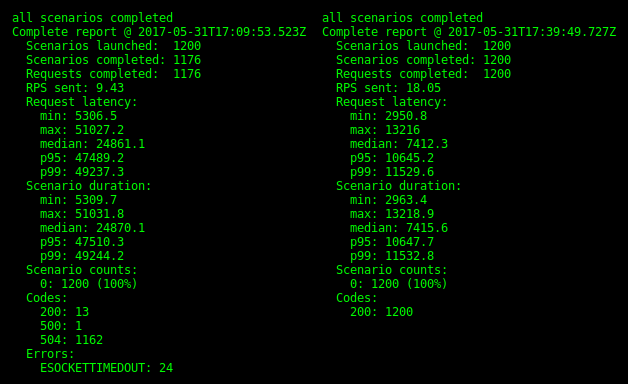
\includegraphics[width=0.9\textwidth]{pen_test.png}
    \caption{Screenshots of two command line outputs showing the results of the REST API being put under high HTTP load. During 60 seconds, the API had to face \emph{1200 requests} of 20 virtual clients created by Artillery. The test on the left was defined to include a single POST request triggering a new build cycle (with a full rebuild option) every time the API accepted a new connection. The results show the following: \emph{24} could not be handled at all, \emph{1162} resulted in gateway timeouts (GitHub blocks), but \emph{13} were handled successfully and returned with a \emph{200 OK} HTTP status code.}
    \label{fig:pen-test}
\end{figure}
%

%% Screenshot of the Mailgun result log
\begin{figure}[h] % h-ere, t-op, b-ottom, p-age
    \centering
    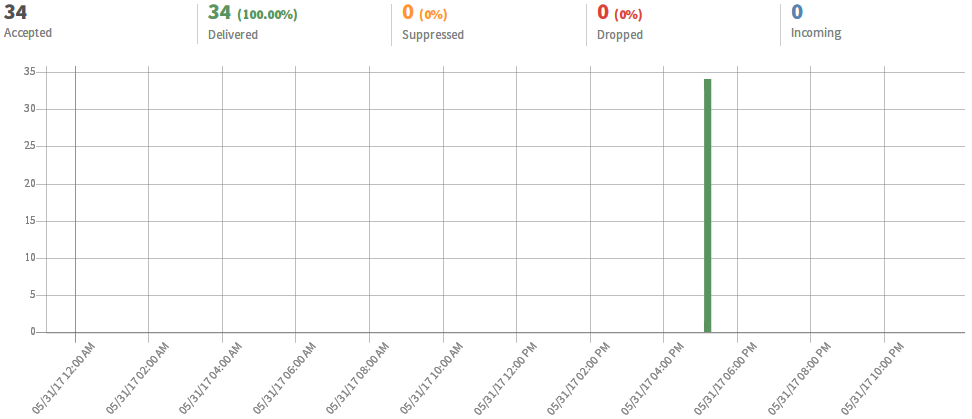
\includegraphics[width=0.9\textwidth]{mailgun_result.png}
    \caption{A screenshot showing the extent of the previous load-test (see fig. \ref{fig:pen-test}) in the Mailgun dashboard. Obviously, the build pipeline was triggered \emph{34} times, leading to the same number of E-Mails being sent. Out of this 34 E-Mails, \emph{8} showed a success message, whereas the others mostly failed due to other concurrent requests deleting the CWD as a preparation step prior to downloading the repository archive.}
    \label{fig:mailgun-result}
\end{figure}
%

\subsection{Load testing}
To evaluate the basic stability while handling multiple concurrent requests, the API was put under a high load test using Artillery\footnote{\url{https://artillery.io} -- Website of Artillery, a load testing toolkit.} (see fig. \ref{fig:pen-test}). Without any load balancing, nor any other high load supporting tool, 1200 POST requests triggered the build pipeline for a total duration of 60 seconds. As explained in the graphic's caption, the penetration test showed a success rate of roughly 1\%, a reasonable minimal response time of about 5 seconds but a terrible maximum response time of 51 seconds.

Of course, this data may not be interpreted as successful result in the first place, but it has to be stated, that the test was run on the endpoint causing the heaviest task in the system and most failure responses were effected by GitHub blocking most requests due to their rate abuse checking system.

The same test running on a much lighter task is showing a different picture; 1200 GET requests for receiving information about the latest build cycle had a response rate of 100\%. The response time ranged from 3 to 13 seconds, which is again a sign to not let a single application handle such an amount of requests without load balancing beforehand. In the end, it is safe to say, that the REST API may handle a reasonable amount of requests quite well on its own (e.g. requests triggered by GitHub webhooks), but consisting of multiple instances may be the best option for handling a significant amount of requests every once in a while.

\section{Caching}
\label{sec:caching}

In terms of caching, the build pipeline is best evaluated when assuming the best possible, as well as the worst possible case. As already explained in ch. \ref{sec:challenges-cachedetermination} on p. \pageref{sec:challenges-cachedetermination}, such scenarios would be on the one hand a commit only containing content changes (e.g. new or modified blog posts) and on the other hand a commit containing a modification of the default template. Since the default template is very likely to act as a dependency of nearly all content files, a full rebuild is inevitable.

\subsection{Initial build}
An initial build is necessary every time a repository was registered using the REST API, or the repository's previous build attempts constantly failed and no successful outcome was produced yet. Not only caring for the required folder structure, a successful build cycle also provides information for a subsequent rendering process by storing its head commit hash value in the build log on the database. Any following build attempt is able to forge upon the last successful build files.

Therefore it is a good advice to have a successful initial build ready as soon as possible, as future build cycles profit from an early render history and a best possible caching structure. By omitting an early registration to the REST API, any initial build cycle in the future will last a significant amount of time longer, due to continuous progression which is not able to make use of any cached file structure.

%% Graphic of MongoDB entries
\begin{figure} % h-ere, t-op, b-ottom, p-age
    \centering
    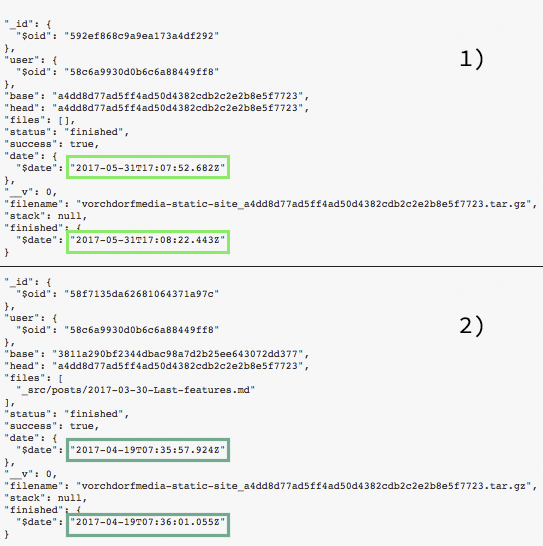
\includegraphics[width=0.9\textwidth]{caching_mongodb.png}
    \caption{Two screenshots of build log entries on the database showing the extent of ideal caching. Example \emph{1)} shows a forced rebuild during the load test (see fig. \ref{fig:pen-test}). Obviously there already happened some successful rendering cycles in the past, as \emph{base} and \emph{head} show the same commit hashes. The build lasted roughly 30 seconds and resulted in a successful archive file.\\
    Example \emph{2)} shows an earlier build, which made use of an available cache. The entry listed in the ``files'' array was the only file, which was rendered and added to the existing file structure. Therefore the build cycle lasted only 4 seconds.}
    \label{fig:caching-mongodb}
\end{figure}
%

\subsection{Caching strategy}
Since caching works most effectively if subsequent commits only contain content changes, the commit culture should be focused towards a content-only development, to make use of a long-lasting series of performant build cycles. Normally, this would be the standard for steady sites containing a significant amount of various information (e.g. FAQ-, support-, or documentation-sites), where constantly changing design decisions are not likely to play an important role. Concerning the need of a templating- or design change, the probably best advice is to collect commits containing such system files for as long as possible before actually merging them into the main branch and causing a longer lasting rebuild task, resulting in a major redesign.

Blogs are also likely to follow this kind of commit pattern, as usually a theme is set once, before subsequent blog posts are published. Using this type of scenario, the extent of ideal caching may be seen on fig. \ref{fig:caching-mongodb}. A rebuild, as well as an initial build at a later time is a lot more time consuming for resulting in a sane file structure, than a selectively rendered build result, which is able to get merged into an existing website root.

Thereby it is not important to check for any existing file structure, if any previously failed build attempt forced a rebuild due to its commit history, as the current build is always able to rely on the rendering result of the last successfully logged attempt.


\chapter{Conclusion}
\label{cha:conclusion}

The main interest for static site generators evolved during my work at a digital performance monitoring company based in Linz, Upper Austria. I was impressed by the simplicity of generating HTML content without having to construct an extensive interface before even getting to the point of actually creating content. One of the major drawbacks although was the idle time I had to face during a rendering cycle.

One of the projects I used to work with was initially based on Jekyll, but with some strong customizations added to the build pipeline setup. Consisting of a reasonable amount of content files, a build cycle sometimes lasted more than 20 minutes -- mostly due to heavy tasks, such as picture resizing, etc\ldots

\paragraph{}
Therefore, this project was originally designed only as supporting tool for local development, but it quickly grew out of hand as I figured out, that this type of development is facing too many limitations. One of the very first approaches was to use the GitHub API, as I had already gained some experience in using it while working on a few projects in the past. Concerning the amount of information needed, and first and foremost where to actually fetch it, GitHub is the best possible tool to use, unless a strictly local solution is preferred. Soon after, it was clear to build something, which is able to act remotely and as automated as possible.

However, the major premise for this project was to provide an unopinionated tool for rendering a website with a caching solution included. Although this may sound fairly understandable in the first place, it soon turned out, that this mixture is also going to be the biggest challenge in finding a suitable way of solving this problem statement.

As a conclusion, I can now say, the most interesting part about my research was not only to find ways to overcome those local performance issues during rebuilds, but also trying to leverage the common workflow in moving as many local tasks to a remote workspace as possible. This should support content authors and developers in focusing on their core jobs by taking unnecessary responsibilities off their hands.

\paragraph{}
Soon after my initial project setup, I was already forced to balance the importance of the core principles and therefore I had to compromise over some of them. First, the project is not as unopinionatedly usable as originally planned, as by all forms of customizability, Metalsmith needs at least a core structure of parameters in its configuration file. To not interfere with the standard configuration file, I designed an adjusted format, by also allowing it to be written in YAML. This especially should support developers switching from Jekyll.

Second, by providing an automated remote workspace, the question of long-term storage has to be reconsidered, as the tar.gz archive currently only gets written to the same file structure the REST API lies in. This saves time by always having the latest version at hand, however, using an external storage like Amazon S3\footnote{\url{https://aws.amazon.com/s3/?hp=tile&so-exp=below} -- Amazon S3 website.}, the file distribution would scale significantly better (especially when using multiple instances in Docker containers, etc\ldots) and is also a lot cheaper in the long run.

Third, the caching algorithm currently appears very basic, as the variety of future repositories cannot be correctly evaluated by now. Therefore it needs some kind of machine learning, which is able to virtualize a dependency graph throughout a single repository (see ch. \ref{sec:chacheimprovement-machinelearning} on p. \pageref{sec:chacheimprovement-machinelearning}). However, this would cover the extent of a project on its own.

\paragraph{}
Lastly it can be said, that the overall performance of the REST API handling different smaller demo projects during my tests was quite the same, as both a repository containing 24 files and a repository containing roughly over 300 files needed little over 30 seconds for an initial build. A much more interesting examination would be testing the REST API in a productive ecosystem, as the ``real'' needs of a comparable development team would be revealed much faster and much more precise. Depending on these informations, future development could be lead towards fields which really matter.

To sum everything up, the outcome is quite the initially expected extent; a proof of concept, which is able to produce a usable website on the one hand, but on the other hand should as well demonstrate the difficulties of providing and running an unopinionated, semi-automated system, which should be able to work with highly diverse source repositories together with as many requests as possible at the same time. This project shows that all of this is possible, if the end user is able to compromise on his expectations and development is pushed further towards a more user-friendly surrounding.
%% verschiedenheit der projekte, unopinionated, begrenztheit der vielfalt, etc..


%%%----------------------------------------------------------
\appendix                                            % Anhang
%%%----------------------------------------------------------

%\chapter{Technische Informationen}
\label{ch:TechnischeInfos}

\newcommand*{\checkbox}{{\fboxsep 1pt%
\framebox[1.30\height]{\vphantom{M}\checkmark}}}

\section{Aktuelle Dateiversionen}

\begin{center}
\begin{tabular}{|l|l|}
\hline
Datum & Datei \\
\hline\hline
\hgbthesisDate & \texttt{hgbthesis.cls} \\
\hline
\hgbDate       & \texttt{hgb.sty} \\
\hline
\end{tabular}
\end{center}




\section{Details zur aktuellen Version}


Das ist eine völlig überarbeitete Version der DA/BA-Vorlage, die
\mbox{UTF-8} kodierten Dateien vorsieht und ausschließlich im PDF-Modus arbeitet.
Der "`klassische"' DVI-PS-PDF-Modus wird somit nicht mehr unterstützt! 

\subsection{Allgemeine technische Voraussetzungen}

Eine aktuelle \latex-Installation mit
\begin{itemize}
	
		\item Texteditor für \mbox{UTF-8} kodierte (Unicode) Dateien,
		\item \texttt{biber}-Programm (BibTeX-Ersatz, Version $\geq 1.5$),
		\item \texttt{biblatex}-Paket (Version $\geq 2.5$, 2013/01/10),
		\item Latin Modern Schriften (Paket \texttt{lmodern}).%
			\footnote{\url{http://www.ctan.org/pkg/lm}, \url{http://www.tug.dk/FontCatalogue/lmodern}}
\end{itemize}


\subsection{Verwendung unter Windows}

Eine typische Installation unter Windows sieht folgendermaßen aus
(s.\ auch Abschnitt \ref{sec:Windows}):
%
\begin{enumerate}
\item \textbf{MikTeX 2.9}%
	\footnote{\url{http://www.miktex.org/} -- \textbf{Achtung:} 
	Generell wird die \textbf{Komplett\-installation} von MikTeX ("`Complete MiKTeX"') empfohlen, 
	da diese bereits alle notwendigen Zusatzpakete und Schriftdateien enthält! 
	Bei der Installation ist darauf zu achten, 
	dass die automatische Installation erforderlicher Packages 
	durch "`\emph{Install missing packages on-the-fly: = Yes}"' ermöglicht wird (NICHT "`\emph{Ask me first}"')!
	Außerdem ist zu empfehlen, unmittelbar nach der Installation von MikTeX mit dem Programm
	\texttt{MikTeX} $\to$ \texttt{Maintenance} $\to$ \texttt{Update} und \texttt{Package Manager} 
	ein Update der installierten Pakete durchzuführen.}
	(zurzeit am einfachsten die 32-Bit Version, da nur diese das Programm \texttt{biber.exe} 
	bereits enthält),
\item \textbf{TeXnicCenter 2.0}%
	\footnote{\url{http://www.texniccenter.org/}}
	(Editor-Umgebung, unterstützt UTF-8),
\item \textbf{SumatraPDF}%
	\footnote{\url{http://blog.kowalczyk.info/software/sumatrapdf/}} 
	(PDF-Viewer),
\end{enumerate}
%
Ein passendes TeXnicCenter-Profil für MikTeX, Biber und Sumatra ist in diesem Paket enhalten
(Datei \verb!_tc_output_profile_sumatra_utf8.tco!). Dieses sollte man zuerst
über \texttt{Build} $\to$ \texttt{Define Output Profiles} in TeXnicCenter importieren.
\textbf{Achtung}: Alle neu angelegten \texttt{.tex}-Dateien sollten in UTF-8 Kodierung gespeichert werden!




\subsection{Verwendung unter Mac~OS}


Diese Version sollte insbesondere mit \emph{MacTeX} problemlos laufen (s.\ auch Abschnitt \ref{sec:MacOs}):
\begin{enumerate}
\item 
	\emph{MacTex} (2012 oder höher).
\item 
	Die Zeichenkodierung des Editors sollte auf UTF-8 eingestellt sein.
\item 
	Als Engine (vergleichbar mit den Ausgabeprofilen in TeXnicCenter) sollte \emph{LaTeXMk} verwendet werden. 
	Dieses Perl-Skript erkennt automatisch, wie viele Aufrufe von \emph{pdfLaTeX} und \emph{Biber} nötig sind. 
	Die Ausgabeprofile \emph{LaTeX} oder \emph{pdfLaTeX} hingegen müssen mehrmals aufgerufen werden, 
	zudem werden hierbei auch die Literaturdaten nicht verarbeitet. Dazu müsste extra die \emph{Biber}-Engine 
	aufgerufen werden, 	die jedoch noch nicht in allen Editoren vorhanden ist.
\end{enumerate}


\begin{comment}
\subsection{Vorteile}
\begin{itemize}
\item PDF wird direkt erzeugt ohne DVI und PS; damit ist angeblich auch die "`Feintypographie"' besser.
\item Die Verwendung von \texttt{SumatraPDF} erlaubt funktionierende Forward- und Inverse-Suche, womit erstmals ein effektiver PDF-Workflow möglich ist.
\item Preview der vollständigen Manuskripts (inklusive Grafiken) ist in PDF viel schneller
als in DVI (mit YAP und Ghostscript für die Grafiken).
\item Grafiken können auch als PDF, PNG oder JPEG direkt eingebunden werden. Bestehende EPS-Grafiken werden automatisch in PDF konvertiert. 
\item Bei eingebundenen Rasterbildern werden (im Unterschied zu \texttt{ps2pdf} in der Default-Einstellung) keine zusätzlichen JPEG-Artefakte erzeugt. 
(Anmerkung: im TC-Ausgabeprofil für \texttt{ps2pdf} ist dafür jetzt die
Option \verb!-dPDFSETTINGS=/prepress! eingestellt -- \verb!=/printer! ist nicht ausreichend!)
\item Die Erzeugung von aktiven Verweisen mit \texttt{hyperref} funktioniert problemlos, mit allen Vorteilen (einschließlich der Zeilenumbrüche in URLs).
\item PDF-Metadaten (zur verbesserten Suche) werden direkt aus den Dokumentendaten durch LaTeX generiert.
\end{itemize}

\subsection{Weitere Neuerungen}
%
\begin{sloppypar}
\begin{itemize}
\item Verwendung des \texttt{epstopdf}-Pakets, wodurch vorhandene EPS-Grafiken (mit denen \texttt{pdflatex} nicht umgehen kann) automatisch in PDF-Dateien konvertiert werden, unter der Annahme, dass \texttt{epstopdf.exe} vorhanden ist. Das ist bei Rasterbildern allerdings nicht zu enpfehlen, weil mit \texttt{epstopdf} die Kompressionsqualität nicht gesteuert erden kann. In diesem Fall ist es besser, die EPS-Dateien (\zB\ mit PhotoShop) direkt in PDFs zu konvertieren oder (noch besser) die Original JPEG- oder PNG-Dateien zu verwenden.
%
\item Unter \texttt{pdflatex} können nun (mit \verb!\includegraphics{}!) neben PDFs auch Bilder im JPEG- oder PNG-Format direkt eingebunden werden. Alle Datei-Extensions der Grafikdateien wurden im Quelltext entfernt.
%
\item 
Verwendung des \textbf{SumatraPDF}-Viewers anstelle von Adobe Acrobat, da Acrobat das Überschreiben der Ausgabedatei blockiert (unter Windows) und forward/inverse Suche schlecht \bzw\ gar nicht unterstützt.
Anweisungen zur Einstellung findet man unter \url{http://www.hehn.biz/Mar/How_to_Sumatra.pdf} -- diese sind auch im beiliegenden TC-Aus\-gabe\-profil implementiert.
%
\item Verwendung des \texttt{pdfsync}-Pakets zur Unterstützung der inversen Suche aus PDF-Dateien.
%
\item Verwendung des \texttt{hyperref}-Pakets zur Aktivierung von Links (Web, Inhaltsverzeichnis, Querverweise, Literatur etc.). Erzeugt auch eine Navigation-Pane.
%
\item PDF-Metadaten werden automatisch aus den Dokumentendaten generiert (durch \texttt{hyperref} möglich).
%
\item Verwendung des \texttt{breakurl}-Pakets, mit dem Zeilenumbrüche trotz \texttt{hy\-per\-ref} auch bei DVI-PS-PDF-Generierung durchgeführt werden. Dadurch sind jetzt auch URLs in Captions und Fußnoten problemlos möglich und auch \verb!\urldef{}! ist nicht mehr erforderlich (entspr.\ Textpassagen in \ref{sec:QuellenangabenInCaptions} entfernen!). 
%
\item Alle bestehenden EPS-Dateien mit Rasterbildern wurden auf Binärkodierung umgestellt, da dies mit der aktuellen MikTeX-Version keine Probleme mehr verursacht. Zusätzlich wurden PNG-Versionen für \texttt{pdflatex} angelegt, sodass keine automatische Umwandlung mit \texttt{epstopdf} erfolgt.
%
\item
Das lästige Problem des übermäßigen vertikalen Abstände in LaTeX-Aufzählungslisten wurde mit dem \texttt{enumitem}-Paket behoben. Alle \verb!\itemsep0pt! Anweisungen im Text wurden entfernt.
%
\item Einbindung des \texttt{cite}-Pakets mit \texttt{noadjust}-Option, womit kein zusätzliches Spacing erzeugt wird.
\end{itemize}
\end{sloppypar}
\end{comment}


\begin{comment}
\section{Einstellungen unter Windows} 
\label{sec:EinstellungAusgabeprofile}

Die folgenden Angaben beziehen sich auf eine bewährte Arbeitsumgebung unter Windows (XP, Win7) mit MikTeX, Sumatra-PDF und TeXnicCenter, mit folgenden Installationspfaden:
%
\begin{quote}
\verb!C:\Program Files (x86)\MiKTeX 2.9\! \\
\verb!C:\Program Files (x86)\SumatraPDF\! \\
\verb!C:\Program Files (x86)\TeXnicCenter\! 
\end{quote}
%
Unter Windows XP liegen die Programme in \verb!C:\Program Files\!.
Falls neuere Versionen dieser Komponenten installiert sind, müssen natürlich die nachfolgend angegebenen Pfade entsprechend modifiziert werden.

\begin{quote}
\textbf{Achtung:} Für MikTeX immer die \textbf{komplette Version} installieren! Das entsprechende Installationsverzeichnis hat aktuell einen Umfang von ca.\ 1.2 GB und enthält etwa 53.200 Dateien 
(typischerweise in \nolinkurl{C:\\Program Files (x86)\\MiKTeX...}).
\end{quote}
\end{comment}

\begin{comment}
\subsection{TeXnicCenter-Ausgabeprofile}
\label{sec:TeXnicCenterUndMikTeX}

TeXnicCenter definiert den Verarbeitungsablauf des LaTeX-Dokuments anhand von Ausgabeprofilen, wobei die oben genannten Komponenten als externe Programme mit entsprechenden Argumenten aufgerufen werden.
Die Einstellung der Ausgabeprofile erfolgt in TeXnicCenter über das Menü
\textsf{Ausgabe}$\rightarrow$\textsf{Ausgabeprofile definieren...} (Abb.\ \ref{fig:techniccenter-profile-latex}). 
Die Profile werden (abhängig von der installierten Software) üblicherweise beim ersten Start von TeXnicCenter durch den zugehörigen "`Wizard"' voreingestellt. 

\begin{figure}
\centering\small
\setlength{\tabcolsep}{0pt}%
\begin{tabular}{c@{~}c}
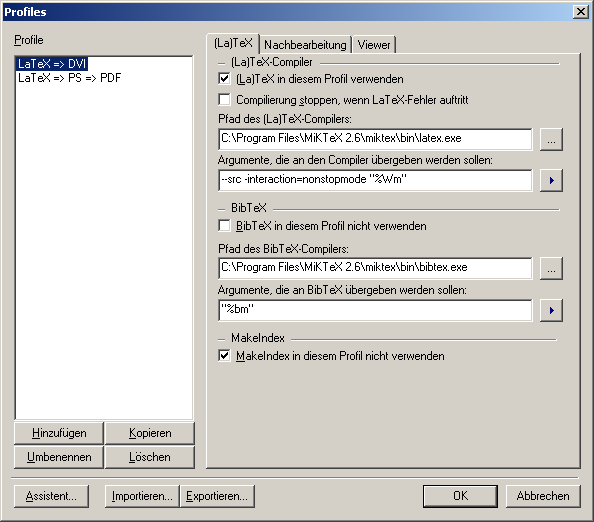
\includegraphics[width=0.49\textwidth]{techniccenter-profile-dvi-26} &
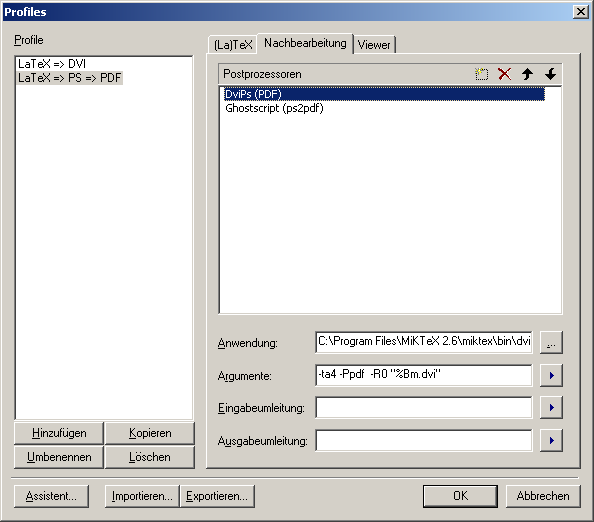
\includegraphics[width=0.49\textwidth]{techniccenter-profile-dvips-26} \\[4pt]
(a) & (b)
\end{tabular}
\caption{Spezifikation der Ausgabeprofile in TeXnicCenter.}
\label{fig:techniccenter-profile-latex}
\end{figure}

In der Datei \verb!tc_output_profiles_sumatra.tco! sind  folgende beiden "`maßgeschneiderten"' Ausgabeprofile für TexNicCenter angelegt (Import über \textsf{Build} $\rightarrow$ \textsf{Define Output Profiles ...}):
\begin{itemize}
	\item \verb!LaTeX => PDF (Sumatra)! -- Standard, direkte Erzeugung von PDF,
	\item \verb!LaTeX => PS => PDF (Sumatra)! -- PDF "`klassisch"' via DVI und PS.
\end{itemize}

\subsubsection{Profil "`\texttt{LaTeX => PDF (Sumatra)}"'}

Das ist das mit diesem Setup normalerweise verwendete Standardprofil.

\paragraph{(La)Tex:}
\begin{itemize}
  \item Path to the (La)TeX compiler: \\
        \begin{small} \verb!C:\Program Files (x86)\MiKTeX 2.9\miktex\bin\pdflatex.exe!\end{small}
  \item Command line arguments to pass to the compiler:\\
\begin{small}
   \verb!-synctex=-1 -interaction=nonstopmode "%pm"!
\end{small}
\end{itemize}

\paragraph{Postprocessor:} 
leer, kein Postprocessor notwendig.

\paragraph{Viewer:}
\begin{itemize}
\item Path of executable: \\
\begin{small}
    \verb!C:\Program Files (x86)\SumatraPDF\SumatraPDF.exe ! \\ 
    \verb!-inverse-search "\"C:\Program Files\TeXnicCenter\TEXCNTR.EXE\" !\\
    \verb!/ddecmd \"[goto('%f','%l')]\""!
\end{small}
%
\item View project's output: \\
\begin{small}
    \checkbox\ Command line argument \\\
    Command: \verb!"%bm.pdf"!
\end{small}
%
\item Forward search:\\
\begin{small}
    \checkbox\ DDE command \\\
    Command: \verb![ForwardSearch("%bm.pdf","%Wc",%l,0)]! \\
    Server: \verb!SUMATRA! \\
    Topic: \verb!Control!
\end{small}
\item Close document before running (La)TeX:\\
\begin{small}
    \checkbox\ Do not close
\end{small}
\end{itemize}


\subsubsection{Profil "`\texttt{LaTeX => PS => PDF (Sumatra)}"'}

Profil ausschließlich für den DVI-PS-Workflow (über DVI und PostScript).

\paragraph{(La)Tex:}
\begin{itemize}
  \item Path to the (La)TeX compiler: \\
        \begin{small} \verb!C:\Program Files (x86)\MiKTeX 2.9\miktex\bin\latex.exe!\end{small}
  \item Command line arguments to pass to the compiler:\\
\begin{small}
   \verb!-synctex=-1 -interaction=nonstopmode "%pm"!
\end{small}
\end{itemize}

\paragraph{Postprocessor:}
\begin{itemize}
  \item DviPS (PDF): \\
        \begin{small} 
        Executable: \verb!C:\Program Files (x86)\MiKTeX 2.9\miktex\bin\dvips.exe! \\
        Arguments: \verb!-ta4 -P pdf -R0 "%Bm.dvi"!
        \end{small}
  \item Ghostscript (ps2pdf):\\
  		\begin{small} 
        Executable: \verb!C:\Program Files (x86)\gs\gs9.04\bin\gswin32c.exe! \\
        Arguments: \verb!-q -dPDFSETTINGS=/prepress -sPAPERSIZE=a4 -dSAFER! \\
         \verb!-dBATCH -dNOPAUSE -sDEVICE=pdfwrite -sOutputFile="%bm.pdf"! \\
         \verb!-c save pop -f "%bm.ps"!
      \end{small}
\end{itemize}

\paragraph{Viewer:}
wie in Profil A. (\texttt{LaTeX => PDF (Sumatra)}).

\section{Tipps und offene Probleme:}

\begin{itemize}
\item \texttt{psfrag} funktioniert nicht mit \texttt{pdflatex} und es gibt auch leider keine Ersatzlösung. 
Wenn man \texttt{psfrag} braucht, dann muss man weiterhin über PostScript 
(\verb!LaTeX => PS => PDF!) arbeiten (was allerdings nunmehr auch mit \texttt{hyperref} kein Problem mehr ist).
%
\item Bei Verwendung des TexWorks-Editors (wird mit MikTeX ausgeliefert) sollte man die Standard-Zeichenkodierung von \emph{Unicode} (utf8) auf \emph{Latin-1} (ISO 8859-1) umstellen.
%
\item Adobe Illustrator kann beim Speichern als PDF die Bounding Box nicht setzen. 
Eine Möglichkeit ist, die Grafik zuerst als EPS zu exportieren und dann mit Acrobat in ein PDF zu konvertieren. 
%
\end{itemize}
\end{comment}



\begin{comment}
\section{Einstellungen für YAP (DVI-Viewer) im DVI-PS-Workflow}
\label{sec:YapEinstellung}

Im Standard-DVI-Viewer YAP lässt sich durch Mausklick auf das DVI-Dokument sehr leicht die zugehörige Stelle im Quelltext finden. Im Normalfall öffnet dann TeXnicCenter das zugehörige \latex-Dokument automatisch an der richtigen Stelle.
Das zugehörige "`Inverse DVI Search"' Kommando sollte sich bereits bei der Installation richtig einstellen.

Falls dies \emph{nicht} funktioniert, kann man in YAP diese Einstellung auch manuell über das Menü \textsf{View}\thinspace$\rightarrow$\thinspace\textsf{Options...} vornehmen, wie in Abb.\ \ref{fig:yap-inverse-search} gezeigt.
In diesem Fall lautet die vollständige Anweisung in "`Command Line"' folgendermaßen:
\begin{center}\footnotesize
\verb!"C:\Program Files (x86)\TeXnicCenter\TEXCNTR.EXE" /ddecmd "[goto('%f', '%l')]"!
\end{center}


\begin{figure}
\centering\small
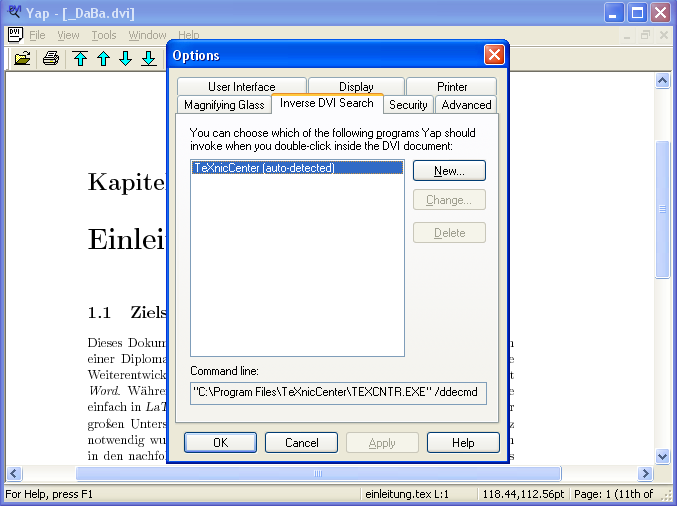
\includegraphics[width=1.0\textwidth]{yap-inverse-search-settings}
\caption{"`Inverse DVI Search"' Einstellung in YAP (über das Menü \textsf{View}\thinspace$\rightarrow$\thinspace\textsf{Options...}).}
\label{fig:yap-inverse-search}
\end{figure}

Latex
C:\Program Files\MiKTeX 2.6\miktex\bin\latex.exe
--src -interaction=nonstopmode "%Wm"

Bibtex
C:\Program Files\MiKTeX 2.6\miktex\bin\bibtex.exe
"%bm"

---

DviPs (PDF)
C:\Program Files\MiKTeX 2.6\miktex\bin\dvips.exe
-ta4 -Ppdf  -R0 "%Bm.dvi"

Ghostscript (ps2pdf)
C:\Program Files\gs\gs8.61\bin\gswin32c.exe
-sPAPERSIZE=a4 -dSAFER -dBATCH -dNOPAUSE -sDEVICE=pdfwrite -dPDFSETTINGS=/prepress -sOutputFile="%bm.pdf" -c save pop -f "%bm.ps"


YAP 
Options -> Inverse Search
"C:\Program Files\TeXnicCenter\TEXCNTR.EXE" /ddecmd "[goto('%f', '%l')]"

\end{comment}

	% Technische Ergänzungen
\chapter{Contents of the CD-ROM}
\label{app:cdrom}

\paragraph{Format:}
		CD-ROM, Single Layer, ISO9660-Format%


\section{PDF files}
\begin{FileList}{/}
%\fitem{_DaBa.dvi} Gesamtdokument (DVI-File, ohne Grafiken)
\fitem{S1510629021_Zarhuber_Thesis.pdf} Master's Thesis with instructions (entire document)%
\end{FileList}

\begin{FileList}{/online}
  \fitem{Hexo 3.2.0-beta.2.pdf} \cite{Chen2015hexorelease}
  \fitem{Hexo debut.pdf} \cite{Chen2012hexodebut}
  \fitem{Hexo Documentation - Setup.pdf} \cite{HexoDocumentationSetup}
  \fitem{JSLint Documentation.pdf} \cite{JSLintDocumentation}
  \fitem{Node.js Documentation.pdf} \cite{NodejsChildProcesses}\cite{NodejsKillProcess}
  \fitem{Overview of Blocking vs Non-Blocking.pdf} \cite{NodejsBlockingNonblocking}
  \fitem{git-diff.pdf} \cite{GitDiff}
  \fitem{git-revert.pdf} \cite{GitRevert}
  \fitem{Introducing Markdown.pdf} \cite{Markdown2004introduction}
  \fitem{Markdown.pdf} \cite{Markdown2004main}
  \fitem{OAuth2orize.pdf} \cite{OAuth2orizeGitHub}
  \fitem{Routing.pdf} \cite{ExpressRouter}
  \fitem{Using middleware.pdf} \cite{ExpressMiddleware}
  \fitem{About pull requests.pdf} \cite{GithubPullRequests}
  \fitem{Basics of Authentication.pdf} \cite{GithubAuthentication}
  \fitem{Mastering Markdown.pdf} \cite{GithubFlavoredMarkdown}
  \fitem{Merging a pull request.pdf} \cite{GithubMergePullRequests}
  \fitem{Resolving a merge conflict using the command line.pdf} \cite{GitConflicts}
  \fitem{Webhooks.pdf} \cite{GithubWebhooks}
  \fitem{Write Scripts for the mongo Shell.pdf} \cite{MongoDBWritingScripts}
  \fitem{Building Technical Documentation with Metalsmith.pdf} \cite{Metalsmith2015technicaldocumentation}
  \fitem{Node based static site generators.pdf} \cite{Mann2012nodestaticsite}
  \fitem{JavaScript reference - Arrow functions.pdf} \cite{MDNArrowFunctions}
  \fitem{Using promises.pdf} \cite{MDNPromise}
  \fitem{Git Projects.pdf} \cite{PancakeGitProjects}
  \fitem{Blogging Like a Hacker.pdf} \cite{PrestonWerner2008jekyll}
  \fitem{GitHub Pages.pdf} \cite{PrestonWerner2008githubpages}
  \fitem{How I Turned Down USD 300,000.pdf} \cite{PrestonWerner2008githublaunch}
  \fitem{Directory structure.pdf} \cite{JekyllDirectoryStructure}
  \fitem{Usage of server-side programming languages for websites.pdf} \cite{W3TechLanguageTrends}
  \fitem{Setting up a Node.js Cluster.pdf} \cite{RobinsonNodeCluster}
  \fitem{Metalsmith Repository.pdf} \cite{MetalsmithRepository}
  \fitem{Building Building Blocks} \cite{Metalsmith2015buildingblocks}
\end{FileList}

\begin{FileList}{/source}
  \fitem{Technical Documentation.pdf} \latex version of the project's README.md
\end{FileList}


\section{Source code}
\begin{FileList}{/source}
  \fitem{v1.0.1.zip} Source code of the project
\end{FileList}


\section{Graphics}
\begin{FileList}{/images}
  \fitem{*.sketch} Source files
  \fitem{*.svg} Vector graphics
  \fitem{*.png} Rendered images \& Screenshots
\end{FileList}
	% Inhalt der CD-ROM/DVD
%\chapter{Chronologische Liste der Änderungen}


\begin{sloppypar}
\begin{description}
%
\item[2002/01/07]
\verb!\newfloat{program}! repariert (auch ohne Chapter). Dank an Werner Bailer!
%
\item[2002/03/06]
Copyright-Notice an internat.\ Standard angepasst. Dank an Karin Kosina!
%
\item[2002/07/28]
"`Studiengang"' $\rightarrow$ "`Diplomstudiengang"'
%
\item[2003/08/24]
Neues Macro: \verb!\Messbox{breite}{hoehe}! -- zur Kontrolle der 
Druckgröße ohne PS-Datei. Erweiterungen für Bakkalaureatsarbeiten
%
\item[2005/04/09]
Diverse Korrekturen: Captions von Tabellen nach oben gesetzt. 
\texttt{caption} auf neue Versionen adaptiert.
\texttt{subfigure} wird nicht mehr verwendet
%
\item[2006/01/20]
Adaptiert zur Verwendung als Praktikumsbericht 
(2.\ Bakk.-Arbeit)
%
\item[2006/03/24]
Fehler in \verb!\erklaerung! beseitigt (Dank an David Schwingenschlögl)
%
\item[2006/04/06]
Verwendung von T1-Fontencoding zur besseren Silbentrennung bei 
Umlauten etc.
%
\item[2006/06/21]
Neu: Bachelorstudiengang / Masterstudiengang.
Literaturverweise auf Bakk-Arbeiten.
\texttt{upquote.sty} eliminiert (Problem mit TS1-Kodierung).
Verwende Komma (statt Punkt) als Trennzeichen in Dezimalzahlen.
%
\item[2006/09/14]
Anmerkungen zum Thema Plagiarismus.
%
\item[2007/07/16]
Ergänzungen für Code-Listings (listings) und Algorithmen 
(\texttt{algorithmicx}).
BiBTeX-Datei aufgeräumt, Verwendung der Literaturformate 
verbessert.
Komma (statt Punkt) als Trennzeichen in Dezimalzahlen wieder 
entfernt.
Verwendung der \texttt{ae}-Fonts eliminiert (\texttt{cm-super} Fonts müssen 
installiert sein, ab MikTeX 2.5). 
Beispiel für Ersetzung in EPS-Dateien mit \texttt{psfrag}.
%
\item[2007/10/04]
Version 5.90: Das Laden der Pakete \verb!inputenc! (Option \texttt{latin}) und 
\verb!graphicx! (Option \texttt{dvips})
aus der Hauptdatei in die \texttt{sty}-Datei übertragen; \texttt{upquote} funktioniert nun.
Paket \texttt{eurosym} ergänzt für Euro-Symbol (Anregung von Andreas 
Doubrava).
Problem mit \texttt{color}-package repariert (gerasterter PDF-Ausdruck).
Hinweise bzgl.\ Literatur ergänzt (\texttt{month}, \texttt{edition}),
BibTeX-Datei gesäubert.
Hinweis zum Einfügen von vertikalem Abstand zwischen Absätzen.
Mathematik aufgeräumt, Verwendung von \texttt{amsmath}, 
Fallunterscheidungen.
Diverse Änderungen bei Tabellen und Programmkode.
Beispiele für BibTeX-Angaben von Spezialquellen: Audio-CDs, 
Videos, Filme. Einbinden von Dateien mit \verb!\include{..}!
Neue Datei: \verb!_SimpleReport.tex! für kurze Reports (Projekte etc.).
%
\item[2007/11/11]
Version 5.91: Hinweise zur Einstellung der Output-Profile in
TexNicCenter, Inverse Search Einstellung in YAP im Anhang.
%
\item[2008/04/01]
Version 6.00beta -- kompletter Umbau!
Auslagerung der Doku\-menten-relevanten Teile in eine eigene 
\emph{class}-Datei (\texttt{hgbthesis.cls}) mit Optionen.
Die neue Style-Datei \texttt{hgb.sty} ist nun unabhängig vom 
Dokumententyp und nicht mehr kompatibel mit älteren Versionen!
Die Liste der Änderungen ist jetzt in der Datei \verb!_ChangeLog.tex!
(DIESE Datei) und diese wird im Anhang eingebunden.
Heading-Style auf Sans Serif geändert (ohne grausliche "`Caps"').
%
\item[2008/05/22]
Neue Vorlage für Technical Reports (Klasse \texttt{hgbreport.cls}).
Spracheinstellung nunmehr mit \texttt{babel}-Paket, Hauptsprache
des Dokuments kann als Option der Klasse angegeben werden.
Sprachumschaltung innerhalb des Dokuments funktioniert nun
richtig. Mit der Sprachoption \texttt{german} wird automatisch die neue deutsche 
Orthographie (\texttt{ngerman}) verwendet.
\texttt{babelbib} wird zur Formatierung des Literaturverzeichnisses
verwendet (neue BibTeX-Style-Optionen!).
Header werden nunmehr mit \texttt{fancyhdr}-Paket erzeugt.
Versionsnummerierung von \texttt{.cls} und \texttt{.sty} Files wird beendet 
(ab jetzt gilt: \emph{Datum} = \emph{Version}). 
%
\item[2008/06/10]
Neues Listing-Environment \texttt{PhpCode}; bei allen Listing-Eviron\-ments ist nun 
\texttt{mathescape=false} (kein Math-Mode nach \verb!$!). 
Bug bei Sprachumschaltung auf \texttt{ngerman} beseitigt.
%
\item[2008/08/15]
Diverse Kleinigkeiten in Literaturangaben überarbeitet (Dank an Norbert Wenzel), Spracheinstellung vereinheitlicht, Umlaute in \texttt{.bib}-Datei ersetzt.
%
\item[2008/10/15] 
Zusätzliche Hinweise zur MikTeX-Installation (Windows) sowie LaTeX unter Mac OS~X und Linux.
Liste der Abkürzungen ergänzt.%
\item[2008/11/15] 
Diverse Schreibfehler korrigiert (Dank an Silvia Fuchshuber). Hinweis auf 
\texttt{sloppypar}-Umgebung.
%
\item[2008/12/09] 
BibTeX-Tools: neuer Hinweis auf JabRef ergänzt, BibEdit entfernt (ist nicht mehr auffindbar).
%
\item[2009/02/09]
\texttt{hgb.sty}: Option "`\texttt{spaces}"' zu \texttt{url}-Package ergänzt (ermöglicht gezielten Zeilenumbruch in URLs). 
Im allgemeinen Setup für \texttt{listings}: \texttt{keepspaces=true};
Obsoletes Environment \texttt{sourcecode} deaktiviert.
Escape-Mode für \texttt{LaTeXCode}-Umgebung geändert.
\verb!_DaBa.tex!: Hinweis auf die Verwendung von \verb!\urldef! für die Angabe von URLs in Captions. \texttt{diplom} (statt \texttt{master}) als Standard-Dokumententyp in \verb!_DaBa.tex! ("`Diplomarbeit"'). Neuer Abschnitt zum Umgang mit ``Quellenangaben in Captions''.
\texttt{literatur.bib}: alle URLs (bisher in \texttt{note}-Einträgen) auf \verb!url={..}! geändert.
%
\item[2009/04/14]
Hinweis zum Einfügen einfacher Anführungszeichen ergänzt.
%
\item[2009/07/18]
Literaturangaben korrigiert und ergänzt.
%
\item[2009/11/27]
Experimentelle Version: Massive Änderungen, Umstieg auf \texttt{pdflatex}.
%
\item[2010/06/15]
Erstes Release der neuen Version mit \texttt{pdflatex}.
\item[2010/06/23]
Konflikt zwischen \texttt{pdfsync}-Package und \texttt{array}-Package (wird relativ häufig benutzt) durch \verb!\RequirePackage[novbox]{pdfsync}! behoben.
Seitenunterkante durch \verb!\flushbottom! fixiert,
variablen Absatzzwischenraum reduziert.
\item[2010/07/27]
Sprache der Erklärungsseite auf "`\texttt{german}"' fixiert (auch wenn die Hauptsprache des Dokuments  Englisch ist). %Datumsproblem - Hinweis von Philipp Winter
\item[2010/12/03]
Anmerkungen und Beispiele zum Zitieren von Gesetzestexten und Videos (Zeitangabe) ergänzt.
Hinweis auf \verb!\nolinkurl{..}! zur Angabe von Dateinamen.
\item[2011/01/29]
Einbau der Creative Commons Lizenz und entsprechender Hinweis in 
Abschnitt \ref{sec:HagenbergEinstellungen}. Neue Makros
\verb!\strictlicense!,
\verb!\cclicense! und
\verb!\license{...}!.
BibTeX-Einträge für Audio-CDs und Filme korrigiert, Beispiel für Online-Video ergänzt.
\item[2011/02/01]
Neues Makro \verb!\betreuerin{..}! zur Angabe einer (weiblichen) Betreuerin. 
%
\item[2011/06/26]
Umstellung der gesamten Literaturverwaltung auf \texttt{biblatex} mit dem Ziel, 
getrennte Abschnitte für verschiedene Kategorien von Einträgen im Quellenverzeichnis
zu ermöglichen. Die Wahl fiel auf \texttt{biblatex} (es gäbe andere Optionen), weil
damit BibTeX weiterhin nur einmal aufgerufen werden muss (und nicht für
mehrere Dateien). Damit verbunden sind allerdings massive Änderungen bei der
Syntax der BibTeX-Felder und es gibt auch mehrere neue Felder.
Aktuell sind 3 Kategorien von Quellen vorgesehen, entsprechende Änderungen in 
\nolinkurl{hgbthesis.cls}. Der klassische BibTeX-Workflow wird aktuell nicht
mehr unterstützt, die Möglichkeit einer künftigen Dok-Option ist aber 
vorgesehen. Das Literatur-Kapitel ist komplett überarbeitet, die .bib-Datei
wurde ausgemistet. Neu ist die Empfehlung zur Aufnahme von Bildquellen
in das Quellenverzeichnis, womit lange URLs in Captions (dort sind keine
Fußnoten möglich) nicht mehr notwendig sind. 
"`Persönliche Kommunikation"' als Literaturquelle entfernt (den Inhalt
von Interviews sollte man direkt im Anhang wiedergeben).
Das verwendete Bildmaterial wurde
erneuert, aktuell werden nur mehr Public Domain Bilder verwendet. 
Das Kapitel "`Hinweise für Word-Benutzer"' wurde endgültig entfernt.
\verb!\flushbottom! wieder auf \verb!\raggedbottom! geändert, um übermäßige 
Abstände zwischen Absätzen zu vermeiden.
%
\item[2012/05/10]
Hinweis auf die in Österreich bislang nicht zulässige Verwendung von "`Masterarbeit"'
entfernt, \texttt{master} ist nunmehr die Default-Dokumentenoption.
Anmerkungen zu lästigen \texttt{biblatex}-Warnungen ergänzt.
Angaben für Windows-Programmpfade auf Win7 angepasst, 
MikTeX 2.9 als Minimalerfordernis.\newline
Überflüssige Makros \verb!\damonat! und \verb!\dajahr! endgültig entfernt, statt
\verb!\abgabemonat! und \verb!\abgabejahr! ist nun das neue Makro
\verb!\abgabedatum{yyyy}{mm}{dd}! vorgesehen (unter Verwendung von internen Zählern).
Zur Formatierung von Datumsangaben wir das \texttt{datetime}-Paket verwendet.
\newline
Neue Fassung der eidesstattlichen Erklärung (inkl.\ englischer Version).\newline
PDF-Suche auf \texttt{synctex} umgestellt (\texttt{pdfsync}-Paket ist veraltet und
wird nun nicht mehr verwendet).
\newline
Die älteren Dateiversionen von \texttt{algorithmicx.sty} und \texttt{alg\-pseudo\-code.sty}
(bisher explizit beigefügt) wurden weggelassen.
\newline
Hinweis auf die \emph{Latin Modern Roman} OTF-Schriften ergänzt.
%
\item[2012/07/21]
Quellenverzeichnis: sprachabhängige Einstellung der Überschriften eingerichtet.
Titel des Quellenverzeichnisses auf "`Quellenverzeichnis"' (DE) \bzw\ "`References"' (EN) 
fixiert. Makro \verb!\MakeBibliography! hat damit keinen erforderlichen Parameter mehr.
%
\item[2012/09/17]
Wegen Änderungen im \texttt{biblatex}-package (Version 1.7, 2011/11/13) die Verwendung von
BibTeX als backend eingestellt (\texttt{backend=bibtex8}).
%
\item[2012/10/13]
Option \texttt{lowtilde} beim URL-package eingestellt (erzeugt \url{~} statt \verb!~!).
%
\item[2012/12/01]
In Abschnitt \ref{sec:FormatierungVonProgrammcode} zusätzliche Code-Umgebungen ergänzt:
\texttt{JsCode},
\texttt{PhpCode},
\texttt{HtmlCode},
\texttt{CssCode},
\texttt{XmlCode}.
%
\item[2012/12/08]
Die Code-Umgebungen in Abschn.\ \ref{sec:FormatierungVonProgrammcode} ergänzt und 
zur Verwendung von optionalen Argumenten erweitert (Hinweise in Abschnitt 
\ref{sec:FormatierungVonProgrammcode} auf die Argumente
\texttt{firstnumber=last} und \texttt{numbers=none}).
Quellenverzeichnis: den Eintragstyp \texttt{@software} für Games empfohlen und im Verzeichnis
der Kategorie \emph{avmedia} zugeordnet (Tab.~\ref{tab:BibKategorien} ergänzt). 
Game-Beispiel (von Manuel Wieser) und zusätzliche Tabelle \ref{tab:QuellenUndEintragstypen}
zur besseren Übersicht eingefügt.
%
\item[2013/05/17]
Wichtigste Änderung ist die vollständige Umstellung auf \textbf{UTF-8} unter Beibehaltung des 
\texttt{pdflatex}-Workflows. 
Damit sind zahlreiche weitere Modifikationen verbunden:
\newline
Alle Dateien (auch \texttt{.cls}, \texttt{.sty} und \texttt{.bib}) wurden auf UTF-8 konvertiert.
Damit sollte es auch keine Probleme mehr mit Umlauten und Sonderzeichen unter MacOS geben.
\newline
Die verwendete Standard-Schriftfamilie ist nun "`Latin Modern"' (\texttt{lmodern}). 
Sie ersetzt die "`CM-Super"' Schriften, mit denen es immer wieder Installationsprobleme gab.
Weiters wird jetzt das \texttt{cmap}-Paket zur besseren Such- und Kopierbarkeit von PDFs verwendet.
\newline
Das \texttt{listings}-Paket wurde durch \texttt{listingsutf8} ersetzt und für Umlaute im Quellcode adaptiert.
Eventuell sind weitere Adaptierungen notwendig.
\newline
\texttt{biber} (min.\ Version 1.5!) wird nun anstatt \texttt{bibtex} (unterstützt keine UTF-8 Dateien) verwendet,
zusammen mit \texttt{biblatex} (Version 2.5).
Die Anweisung \verb!\bibliography! wird (wieder) verwendet, allerdings nun in der Präambel,
um die \texttt{.bib}-Datei im Fileverzeichnis anzuzeigen.
\newline
Das Makro \verb!\C! (für die Menge der komplexen Zahlen \Cpx) musste wegen Problemen in der T1-Kodierung
ersetzt werden und heißt nun \verb!\Cpx!. Die Makros 
\verb!\R!, \verb!\Z!, \verb!\N!, \verb!\Q! und \verb!\Cpx! können nun auch außerhalb des Mathematik-Modus verwendet werden.
\newline
Der DVI-PS-PDF Workflow wird ab dieser Version überhaupt nicht mehr unterstützt. 
Damit ist auch das \texttt{psfrag}-Paket nicht mehr verwendbar. Entspechende Hinweise 
wurden aus dem Text entfernt.
\newline
\texttt{hyperref} wurde auf UTF-8 umgestellt.
Die grässlichen Standard-Rahmen und Farben der automatischen \texttt{hyperref}-Links wurden entfernt \bzw\ durch 
dezentere Farben ersetzt. Dadurch wird auch die Screen-Version der PDFs wieder lesbar.
\newline
Im Quellenverzeichnis wurde versuchsweise die \texttt{backref}-Option aktiviert. 
Damit werden bei allen Einträgen auch die zugehörigen Zitierstellen angegeben
(erscheint durchaus sinnvoll).
\newline
Die bisherigen Korrekturen zur \texttt{biblatex}-Formatierung wurden entfernt, 
alles arbeitet nun mit Standard-Einstellungen. Die ursächlichen Probleme in \texttt{biblatex}
scheinen in der aktuellen Version behoben zu sein.
\newline
Das Output-Profil für TeXnicCenter wurde für den neuen Workflow mit \texttt{biber} adaptiert und liegt nun in
\nolinkurl{_tc_output_profile_sumatra_utf8.tco}.
\newline
Das Windows-Script \verb!_clean.bat! wurde entfernt, da TeXnicCenter nun ein eigenes "`Clean Project"'-Kommando aufweist (in "`Build"').
\newline
Allgemeine Einstellungen zu \emph{headings} und \emph{biblatex} wurden aus der Datei \texttt{hgbthesis.cls} entfernt und in 
\texttt{hgbheadings.sty} \bzw\ \texttt{hgbbib.sty} verlagert. Diese können nun unabhängig verwendet werden (s.\ Beispiel in 
\texttt{\_TermReport.tex}).
\newline
Die Klassen-Datei \texttt{hgbtermreport.cls} wurde eliminiert, das Dokument \texttt{\_TermReport.tex} basiert nunmehr
auf der generischen LaTeX-Klasse \texttt{report}  und verwendet keine eigene \texttt{.cls} Datei mehr.
%
\item[2014/11/05]
Neu: Logo auf der Frontseite bei allen Dokumententypen. Dazu gibt es ein neues Kommando
\verb!\logofile{pic}!, wobei \verb!pic! der Name eine PDF-Datei im
Verzeichnis \verb!images/! ist. Falls \emph{kein} Logo erwünscht ist, 
kann man die Zeile einfach weglassen oder durch \verb!\logofile{}! ersetzen.
\newline
\texttt{hyperref}-Einstellungen: Einfärbung der Links wieder entfernt (\texttt{colorlinks = false}), weil beim Druck
nicht abschaltbar. Stattdessen einheitliche (dezente) Rahmen für alle Linkarten.
Zahlreiche Tippfehler eliminiert (Dank an Daniel Karzel).
\newline
Wegen eines Bugs in \texttt{biblatex 1.9} wurden die expliziten Abteilungen (\verb!\-!) in \texttt{literatur.bib}
vorübergehend entfernt (mit entsprechenden Folgen im Ergebnis). Der Bug soll in \texttt{biblatex 2.0} (derzeit noch
nicht verfügbar) behoben sein.
\newline
Package \texttt{color} auf \texttt{xcolor} geändert. In \texttt{hgb.sty} neues "`Convenience-Makro"' \verb!\etc! ergänzt.
Output-Profil für TeXnicCenter/SumatraPDF (Windows) repariert, forward/inverse Search funktioniert nun
(Datei \verb!_tc_output_profile_sumatra_utf8.tco!).
%
\item[2015/04/28]
Paket \texttt{subdepth} (zur verbesserten Platzierung von Sub- und Superscripts) 
in hgb.sty ergänzt.
%
\item[2015/07/14]
Hinweis und Abhilfe für die (nicht automatische) Silbentrennung in zusammengesetzten Wörtern.
Neu in \texttt{hgbheadings.sty}: \verb!\RequirePackage[raggedright]{titlesec}! verhindert Blocksatz
in Section-Überschriften (sehr unschön bei längeren Überschriften). 
Neu (in Abschn.~\ref{sec:GraphicOverlays}): Beispiel für die Verwendung des \texttt{overpic}-Pakets
zur Annotierung von importierten Grafiken (verwendet zudem das \texttt{pict2e}-Paket).
%
\item[2015/08/03]
Logo-Datei auf \texttt{logo.pdf} umbenannt.
\item[2015/09/17]
Anweisung \verb!\RequirePackage[utf8]{inputenc}! in die Doku\-menten\-dateien (\texttt{\_xxx.tex})
verschoben (auf Anregung von Markus Kohm: "`\ldots für die Verwendung von lualatex oder xelatex 
ist die Anweisung in hgb.sty störend, da bei diesen beiden aufgrund der nativen utf8-Unterstützung 
\texttt{inputenc} keinesfalls verwendet werden darf"').
\item[2015/09/19]
\texttt{hgb.sty} aufgeräumt.
Makros \verb!\@savesymbol! und \verb!\@restoresymbol! aus \texttt{hgb.sty} entfernt
(wurden nicht mehr verwendet; ggfs.\ Paket \texttt{savesym} als Ersatz).
Makro \verb!\optbreaknh! (optional break with no hyphen) auf \verb!\obnh! umbenannt.
Teile von \texttt{hgb.sty} in neue Dateien \texttt{hgbabbrev.sty} (div.\ Abkürzungen)
und \texttt{hgblistings.sty} (Code-Listings) verschoben.
Hintergrundtönung der Code-Listings heller (auf 5\% Grau) eingestellt.
Layout: \verb!\textfraction! auf 0.1 (statt fehlhafterweise 0.01) eingestellt.
\texttt{hgbbib.sty}: \verb!\clearpage! am Beginn des Quellenverzeichnisses entfernt
(für \texttt{article}-Template).
\item[2015/09/19]
Alle \texttt{.cls} und \texttt{.sty} Dateien sind jetzt ANSI-codiert (Header eingefügt), wie
laut CTAN-Richtlinien vorgesehen. Umlautzeichen wurden durch Makros ersetzt.
Nur \texttt{hgblistings.sty} ist weiterhin UTF-8 (wegen notwendiger literaler Umlaute).
\verb!\RequirePackage[utf8]{inputenc}! steht sonst nur mehr am Beginn
der jeweiligen (\texttt{.tex}) Haupttextdatei.
\item[2015/10/29]
Verwendung von "`In:"' im Quellenverzeichnis vor \texttt{article}-Einträgen
(Eigenart von biblatex) durch passendes Makro in \texttt{hgbbib.sty} unterbunden 
(Dank an S.\ Dreiseitl).
\item[2015/11/04]
Hinweise in Abschnitt \ref{sec:Software} auf TeXstudio unter Windows, Mac OS und Linux.
Release-Ausgabe.
\item[2015/12/08]
Source Directories neu strukturiert in \texttt{frontmatter}, \texttt{chapters}, 
\texttt{appendix}.
\item[2016/06/09]
Bibliography-Aliases für die Quellentypen
\texttt{video}, \texttt{movie}, \texttt{audio} und \texttt{software}
eingefügt (in \texttt{hgbbib.sty}) -- unterbindet Warnungen wegen
fehlender biblatex-Driver.
\item[2016/06/11]
Repository portiert auf GitHub (SourceForge eingefroren).  
Overleaf als experimentelle online LaTeX-Umgebung.
Hauptdateien umbenannt (auf \texttt{\_thesis}, \texttt{\_praktikum}, etc.).
\end{description}
\end{sloppypar}




%\section*{To Do} 
%\begin{itemize}
%\item Inkscape
%\item biblatex Bib-Driver für audio, video etc. ergänzen.
%\item Mathematik umbauen, typische Fehler stärker berücksichtigen (ua. Leerzeilen vor/nach Gleichungen).
%\item Literaturempfehlungen zum Schreiben von Diplomarbeiten
%\item Hinweise für Literatursuche (Bibliotheksverbund, CiteSeer,...)
%\end{itemize}





	% Chronologische Liste der Änderungen
%\chapter{\latex-Quellkode}
\label{app:latex}

\section*{Hauptdatei {\tt\_DaBa.tex}}

\begin{footnotesize}
\verbatiminput{_DaBa.tex}
\end{footnotesize}


%\vspace*{2cm}
\hrule
\hrule

\paragraph{Anmerkung:}
Das sollte nur ein \emph{Beispiel} für die Einbindung von Quellcode
in einem Anhang sein. Der \latex-Quellkode der eigenen
Abschlussarbeit ist meist \emph{nicht} interessant genug, um ihn hier
wiederzugeben!

	% Quelltext dieses Dokuments

%%%----------------------------------------------------------
\MakeBibliography                        % Quellenverzeichnis
%%%----------------------------------------------------------

%%% Messbox zur Druckkontrolle ------------------------------
\chapter*{Messbox zur Druckkontrolle}



\begin{center}
{\Large --- Druckgröße kontrollieren! ---}

\bigskip

\Messbox{100}{50} % Angabe der Breite/Hoehe in mm

\bigskip

{\Large --- Diese Seite nach dem Druck entfernen! ---}

\end{center}



%%%----------------------------------------------------------
\end{document}
%%%----------------------------------------------------------
